\documentclass[diss,oneside]{iiufrgs}
%\documentclass[diss,oneside]{iiufrgs}
% um tipo específico de monografia pode ser informado como parâmetro opcional:
%\documentclass[tese]{iiufrgs}
% monografias em inglês devem receber o parâmetro `english':
%\documentclass[diss,english]{iiufrgs}
% a opção `openright' pode ser usada para forçar inícios de capítulos
% em páginas ímpares
% \documentclass[openright]{iiufrgs}
% para gerar uma versão somente-frente, basta utilizar a opção `oneside':
% \documentclass[oneside]{iiufrgs}
\usepackage[T1]{fontenc}        % pacote para conj. de caracteres correto
\usepackage[utf8]{inputenc}     % pacote para acentuação
\usepackage[alf]{abntcite}		% pacote para as referencias da abnt nao numerica
\usepackage{graphicx}           % pacote para importar figuras
\usepackage{times}              % pacote para usar fonte Adobe Times
\usepackage{color}              % pacote para usar \textcolor
\usepackage{xcolor,colortbl}    % pacote para usar cores nas tabelas
\usepackage{listings}       	% pacote para usar listagens/listing
\usepackage{rotating}			% rotacionar textos
\usepackage{multirow}			% textos usando mais de uma linha
%\usepackage{mathptmx}          % p/ usar fonte Adobe Times nas fórmulas
\usepackage{wrapfig}			% posiciona elementos de maneira fluante
\usepackage{url}

% Use todo para anotar algo para ver depois
% Criando comando \todo{algo}
\newcommand{\todo}[1] {\footnote{TODO #1}\marginpar{\textcolor{red}{\textbf{TODO}}}}
%\newcommand{\todo}[1] {}
% Use dev para anotar algum comprometimento
\newcommand{\dev}[0] {\marginpar{\textcolor{blue}{\textbf{IMPL}}}}
%\newcommand{\dev}[0] {}

%Citacoes possiveis
%\cite{ortony1988cse} - parenteseses
%\citeonline{ortony1988cse} - texto e parenteses so o ano\\
%\citeauthoronline{ortony1988cse} - so os autores sem ano\\
%\citeyear{ortony1988cse} - so o ano
%\citeauthor{ortony1988cse} - so os autores e sem o 'e'
%atalhos para as citacoes no texto
\newcommand{\citet}{\citeonline}
\newcommand{\jason}{\emph{Jason}}

% Traduzindo Listing
\renewcommand{\lstlistingname}{Listagem}
\renewcommand{\lstlistlistingname}{Lista de Listagens}

%
% Informações gerais
%
\title{MARO: Um modelo de emoções usando ontologia}

\author{Lucca}{Ricardo Rodrigues}
% alguns documentos podem ter varios autores:
%\author{Flaumann}{Frida Gutenberg}

% orientador e co-orientador são opcionais
\advisor[Prof.~Dr.]{Bordini}{Rafael Heitor}
%\coadvisor[Prof.~Dr.]{Meu}{Seila Ainda}

% a data deve ser a da defesa; se nao especificada, são gerados mes e ano correntes
%\date{fevereiro}{2011}

% o nome do curso pode ser redefinido (ex. para TCs)
%\course{Curso de Especialização em Cachaça}

% o local de realização do trabalho pode ser especificado (ex. para TCs)
% com o comando \location:
%\location{Itaquaquecetuba}{SP}

% itens individuais da nominata podem ser redefinidos com os comandos
% abaixo:
% \renewcommand{\nominataReit}{Prof\textsuperscript{a}.~Wrana Maria Panizzi}
% \renewcommand{\nominataReitname}{Reitora}
% \renewcommand{\nominataPRE}{Prof.~Jos{\'e} Carlos Ferraz Hennemann}
% \renewcommand{\nominataPREname}{Pr{\'o}-Reitor de Ensino}
% \renewcommand{\nominataPRAPG}{Prof\textsuperscript{a}.~Joc{\'e}lia Grazia}
% \renewcommand{\nominataPRAPGname}{Pr{\'o}-Reitora Adjunta de P{\'o}s-Gradua{\c{c}}{\~a}o}
% \renewcommand{\nominataDir}{Prof.~Philippe Olivier Alexandre Navaux}
% \renewcommand{\nominataDirname}{Diretor do Instituto de Inform{\'a}tica}
% \renewcommand{\nominataCoord}{Prof.~Carlos Alberto Heuser}
% \renewcommand{\nominataCoordname}{Coordenador do PPGC}
% \renewcommand{\nominataBibchefe}{Beatriz Regina Bastos Haro}
% \renewcommand{\nominataBibchefename}{Bibliotec{\'a}ria-chefe do Instituto de Inform{\'a}tica}
% \renewcommand{\nominataChefeINA}{Prof.~Jos{\'e} Valdeni de Lima}
% \renewcommand{\nominataChefeINAname}{Chefe do \deptINA}
% \renewcommand{\nominataChefeINT}{Prof.~Leila Ribeiro}
% \renewcommand{\nominataChefeINTname}{Chefe do \deptINT}

% A seguir são apresentados comandos específicos para alguns
% tipos de documentos.

% Relatório de Pesquisa [rp]:
% \rp{123}             % numero do rp
% \financ{CNPq, CAPES} % orgaos financiadores

% Trabalho Individual [ti]:
% \ti{123}     % numero do TI
% \ti[II]{456} % no caso de ser o segundo TI

% Trabalho de Conclusão [tc]:
% além de definir explicitamente o nome do curso (\course) e o local
% de realização (\location), é necessário redefinir a nominata,
% pois as informações necessárias dependem do curso. Ex.:
%\renewcommand{\nominata}{
%        UNIVERSIDADE FEDERAL DO RIO GRANDE DO SUL\\
%        Reitora: Prof\textsuperscript{a}.~Wrana Maria Panizzi\\
%        Pró-Reitor de Ensino: Prof.~José Carlos Ferraz Hennemann\\
%        Diretor do Instituto de Informática: Prof.~Philippe Olivier Alexandre Navaux\\
%        Coordenador do curso: Prof.~Seu Creysson\\
%        Bibliotecária-chefe do Instituto de Informática: Beatriz Regina Bastos Haro
%}

% Monografias de Especialização [espec]:
% \espec{Redes e Sistemas Distribuídos}      % nome do curso
% \coord[Profa.~Dra.]{Weber}{Taisy da Silva} % coordenador do curso
% \dept{INA}                                 % departamento relacionado

%
% palavras-chave
% iniciar todas com letras minúsculas, exceto no caso de abreviaturas
%
\keyword{agentes virtuais}
\keyword{programação de agentes}
\keyword{simulação}
\keyword{computação afetiva}
\keyword{modelo OCC}
\keyword{ontologia}

%
% inicio do documento
%
\begin{document}

% folha de rosto
% às vezes é necessário redefinir algum comando logo antes de produzir
% a folha de rosto:
% \renewcommand{\coordname}{Coordenadora do Curso}
\maketitle

%% dedicatoria
\clearpage
\begin{flushright}
\mbox{}\vfill
{\sffamily\itshape
``If I have seen farther than others,\\
it is because I stood on the shoulders of giants.''\\}
--- \textsc{Sir~Isaac Newton}
\end{flushright}

%% agradecimentos
\chapter*{Agradecimentos}
Agradeço ao \LaTeX\ por não ter vírus de macro\ldots


\tableofcontents % sumario
%% lista de abreviaturas e siglas
% o parametro deve ser a abreviatura mais longa
\begin{listofabbrv}{IHC}
		\item[AOP] \underline{A}gent \underline{O}riented \underline{P}rogramming
		\item[ASL] \underline{A}gent\underline{S}peak \underline{L}anguage
		\item[BDI] \underline{B}elief-\underline{D}esire-\underline{I}ntention
        \item[IHC] \underline{I}ntera\c{c}\~{a}o \underline{H}omem-\underline{C}omputador
        \item[OCC] \underline{O}rtony \underline{C}lore e \underline{C}ollins
		\item[OWL] \underline{O}ntology \underline{W}eb \underline{L}anguage
		\item[UEM] \underline{U}rban \underline{E}nvironment \underline{M}odel
        \item[UML] \underline{U}nified \underline{M}odeling \underline{L}anguage
        \item[XML] e\underline{X}tensible \underline{M}arkup \underline{L}anguage

\end{listofabbrv}


%
%% LISTA DE SIMBOLOS
%% o parametro deve ser o simbolo mais longo
%%\begin{listofsymbols}{$\alpha\beta\pi\omega$}
%%       \item[$\sum{\frac{a}{b}}$] Somatório do produtório
%%       \item[$\alpha\beta\pi\omega$] Fator de inconstância do resultado
%%\end{listofsymbols}
%
%%\listoffigures % lista de figuras, se houver mais de 3
%%\listoftables % lista de tabelas, se houver mais de 3
%%\lstlistoflistings % lista de listagens, se houver mais de 3
%
%\definecolor{darkgray}{rgb}{0.95,0.95,0.95}
%\lstset{backgroundcolor=\color{darkgray}}
%\lstset{numbers=left, basicstyle=\scriptsize\ttfamily, numberstyle=\tiny, stepnumber=2, numbersep=5pt}
%
%%\chapter*{Assinaturas}

	\vspace{3cm}

   \begin{center}
        \rule{8cm}{.1mm} \\ Orientador: Prof.~Dr.~Rafael Heitor Bordini
    \end{center}

	\vspace{3cm}

   \begin{center}
        \rule{8cm}{.1mm} \\ Aluno: Ricardo Rodrigues Lucca
    \end{center}


%
%% resumo na língua do documento
\begin{abstract}
Este trabalho apresenta um \emph{framework} que permite aos agentes perceberem
suas próprias emoções. Ele foi feito em \emph{Java} e usa a plataforma
multi-agente \emph{Jason}, sendo que estende a base de crenças da última a fim
de utilizar à ontologia afetiva desenvolvida. Além disso, o ambiente foi
construído a partir de uma base de conhecimento que descreve rotinas.
Adicionalmente, um mecanismo de avaliação das emoções baseando-se nas anotações dos
objetos foi construído apoiado por uma ontologia de preferência sobre essas
anotações. Dessa forma, aplicações de entretenimento poderiam utilizar o
sistema ou as bases de conhecimento apresentadas para diferentes propósitos. A criação de
um mapa onde os personagens atuam, a criação da rotina de cada personagem e
suas preferências são alguns exemplos de utilizações. Para validação desse
desenvolvimento, dois exemplos foram construídos. O primeiro exemplo com a
finalidade principal de demonstrar que o modelo afetivo atingiu a maior parte
dos grafos afetivos. Enquanto, o segundo usa apenas grupo emotivo e serve para
demonstrar a utilização conjunta de todas as ontologias apresentadas.
\end{abstract}

%Example:
%http://www.sbgames.org/sbgames2011/proceedings/sbgames/papers/comp/full/11-92076_2.pdf
%1º, o que é o trabalho
%2º, o que uso e para que
%3º, para que posso utiliza-la
%4º, foi falado que um experimento para validar a arquitetura foi criado

% resumo na outra língua
% como parametros devem ser passados o titulo e as palavras-chave
% na outra língua, separadas por vírgulas
%\begin{englishabstract}{Maro: An emotional model using ontology}{virtual
%agents, programming, agents, simulation, affective computing, OCC's model, ontology}
%This work presents a framework built to work with Jason's platform
%\cite{bordini-jason} to allow agents acknowledge their own emotions. This work have
%been developed in \emph{Java} and extended the belief base from agent of
%platform to utilize an developed ontology based on the affective model
%\cite{ortony1988cse}. For so the development of a belief base permits an agent
%perceive emotions based on your appraisal of environment and conclude new
%beliefs. In addition, an ontology to make the schedules of agents and to make
%yours preferences about annotations on belief were developed. So,
%entertainment applications and games could use the three ontologies together
%to create a map of the city, to create schedules or routines of each
%agent and to give preferences about annotations used in beliefs that came from
%environment. Finally, to validate the framework has been developed an
%soccer's application to demonstrate many emotions from affective model.
%\end{englishabstract}
 % inclui o resumo da lingua nativa e estrangeira

\definecolor{darkgray}{rgb}{0.95,0.95,0.95}
\lstset{backgroundcolor=\color{darkgray}}
\lstset{numbers=left, basicstyle=\scriptsize\ttfamily, numberstyle=\tiny, stepnumber=2, numbersep=5pt}

%% aqui comeca o texto propriamente dito
%% TODO: versoa anterior
%\chapter{Introdução}

Ontologia foi caracterizada como o estudo da existência, desde Aristóteles,
por estar interessada em descrever todas as coisas existentes e as relações
que existem entre elas. Atualmente, essa forma de representar o domínio do
conhecimento tem se tornado popular na computação por causa da independência
de sistema oferecida.

Segundo \citet{gruber1993translation}, uma ontologia é uma especificação explícita do
domínio sendo tratado. Além disso, ele aplica esse conceito em sistemas
baseados em conhecimento onde o domínio é representado por um formalismo
declarativo e o conjunto de conceitos e relações forma o vocabulário usado
pelo sistema. Esse vocabulário provém um conjunto de termos bem formados para
o sistema trabalhar.
%
Entretanto \citet{ontoly2004Approach}, definiu ontologia como uma representação
do conhecimento usado para capturar outras informações ou conhecimentos sobre
o assunto. Atualmente, ontologias são vistas como um entendimento comum e
compartilhado de um domínio que pode ser utilizado na comunicação entre
máquinas ou entre pessoas \cite{wks2008towards}.

O presente trabalho foi baseado na linguagem OWL (\emph{Ontology Web
Language}). Essa linguagem foi regulamentada pela W3C\footnote{Ver
\url{http://www.w3.org/standards/semanticweb/ontology}.}, orgão internacional
que regulamenta padrões na Web, para ser usada na \emph{Web} Semântica.
Essa linguagem foi criada em 2002 com o proposito de criação de ontologias e
trabalha com a hipótese de mundo aberto, isto é, nada é afirmado por não ser
dito. Infelizmente, para a W3C não há uma distinção clara entre vocabulário e
ontologia.

A linguagem OWL permite a especificação de conceitos e não de suas instâncias.
Sendo assim, não é possivel descrever uma regra simples como um conceito de
igualdade onde duas relações distintas tem que chegar na mesma instância
final. %Outro exemplo, o conceito de tios que são os irmãos de meus pais não é
%possível ser feita na OWL. A versão 2 da OWL permite a descrição do conceito
%de tios, porém o conceito de igualdade permanece impossível.
%
A linguagem SWRL (\emph{Semantic Web Rule
Language})\footnote{Mais detalhes \url{http://www.w3.org/Submission/SWRL/}.}
recomendada pela W3C permite escrever regras lógicas que melhoram a
precisão dos conceitos sendo descritos porque permite lidar com as suas
instâncias. Dessa forma, a SWRL supri uma falta até então não tratada pela
linguagem OWL e, por isso, seu uso em conjunto é extremamente poderoso. Essas
duas linguagens juntas permitem a escrita do conceito de igualdade descrito
anteriormente.

A ferramenta \emph{Protege}\footnote{Mais informações, consulte \url{http://protege.stanford.edu}.}
em sua versão 4.1 suporta a linguagem OWL 2 juntamente com a SWRL. Ha suporte
aos raciocinadores chamados \emph{FaCT++}, \emph{HermiT} e \emph{Pellet}.
O raciocinador é uma peça importante porque é através dele que a ontologia
será questionada, isto é, somente com um raciocinador ativo é possível saber
se uma instância pertence a determinado conceito. O raciocinador
\emph{Pellet}\dev{} é o que esta sendo utilizado pelo presente autor por
seu excelente suporte a explicações de inconsistência.

A área da computação que estuda as emoções é denominada Computação Afetiva por
\citet{Pic98}. As emoções, segundo \citet{damasio2004erro}, podem ser divididas
entre primárias (não-cognitivas) e secundárias (cognitivas). As emoções
primárias surgem a partir de reações a determinados estímulos e são geradas
rapidamente. Já as emoções secundárias são aprendidas ao longo da nossa vida,
isto é, são geradas por uma avaliação de uma situação de acordo com nossos
objetivos e valores morais. Entretanto, essa divisão ainda não esta
consolidada porque o fato de haver menos atividade cognitiva não quer dizer
que esta atividade não exista.

\citet{bates1994role} foi um dos primeiros a trabalhar na utilização de
emoções na área de animação. Nessa área, o estudo do comportamento humano é
realizado visando realizar a imitação das ações humanas. Assim, simulando
essas atitudes de uma pessoa de tal maneira que pareça possuir vida própria.
Seu trabalho utilizou o modelo de emoções proposto por \citet{ortony1988cse}.
Esse modelo fundamenta ao todo 22 emoções diferentes divididos em três
formas de percepção: ações, eventos e objetos.

%\begin{figure*}
%  \centering
%    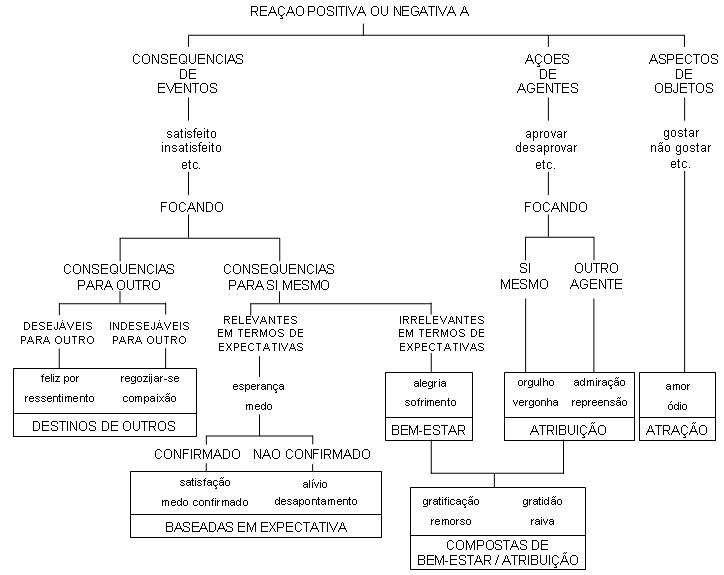
\includegraphics[width=100mm]{figuras/pontarolo_occ.png}
%  \caption{Modelo OCC adaptado de \cite{pontarolo2008modelagem}.}
%  \label{fig:occ_model_original}
%\end{figure*}

A Figura~X\footnote{removido por agora} mostra uma visualização da estrutura
lógica das emoções. As emoções no modelo de \citet{ortony1988cse} já
encontram-se agrupadas em grupos por estarem utilizando regras semelhantes ou
próximas. Esses grupos são representados pelo quadrados e nome do grupo é dado
na parte inferior, assim o ramo de objetos que julga a atração de um indivíduo
com alguma outra coisa (agente ou objeto) possui o grupo de Atração. O ramo de
ações julga a responsabilidade de um agente sobre suas ações e o ramo de
eventos julga a consequência de eventos ou ações desempenhadas. Desse ramo,
o grupo Destinos de outros julga sempre algum outro agente que não é aquele
que esta fazendo a avaliação. Além disso, o grupo denominado Compostas de
Bem-Estar/Atribuição junta os grupos de Bem-Estar (consequência de um evento
sem expectativa) com Atribuição (responsabilidade).

O presente trabalho pretende estudar diferentes ontologias do modelo afetivo
\cite{benta2007ontology,wks2008towards,springerlink:10.1007/978-3-642-01639-448,lera2009semantic}
visando o entendimento destas e suas diferenças. Entretanto, nenhum trabalho propôs
a junção de uma ontologia afetiva com uma humanos virtuais
\cite{Rojas:2006:IRM:1174429.1174442,Gutierrez:2007:OVH:1229160.1229164} com
uma que explique como tratar as percepções do ambiente.

 % ou tambem motivacao
%\chapter{Estado da Arte}

\todo{rever}
%A presente seção se encontra divida em uma introdução a programação de
%agentes na seção~\ref{AOP}, onde é discutido o paradigma e os termos agentes
%e personagens. Na seção~\ref{CA:1} a área de computação afetiva é
%apresentada.  O conceito de ontologia é debatido na seção~\ref{onto} e os
%trabalhos relacionados são apresentados na seção~\ref{TR}.

\section{Conceitos de Agente}

\citet{laird2001human} afirmam que a pesquisa em Inteligência Artificial tem
sido fragmentada em muitas áreas especializadas e, assim, algoritmos
específicos e mais eficientes podem ser criados.
%
Há várias definições do conceito de Agente, por exemplo
\cite{shoham1993agent,roadmap,fatemeh2009multi}. \citet{shoham1993agent}
propõe que Agente é uma entidade definida por componentes mentais como
crenças, habilidades, escolhas e comprometimentos.

\citet{franklin1997agent} define um agente através das características que a
entidade deve apresentar.  Atualmente, o menor conjunto comumente aceito
dessas características é composto por três conceitos principais: (i)
Autonomia; (ii) Sociabilidade; (iii) Situacionalidade.
\citet{roadmap,fatemeh2009multi} concordam que autonomia é quando um Agente
toma suas próprias decisões independente de qualquer outra entidade do sistema
ou, ainda, da intervenção diretas de seres humanos. A característica de
sociabilidade permite flexibilidade na execução das tarefas, através da
interação com outros agentes que estejam presentes no sistema. A última,
permite que o agente situe-se em um ambiente dinâmico interagindo com o mesmo
através de algum tipo de sensor ou atuador.

\citet{ingrand1992architecture} indicam que entidades autônomas podem ter a
capacidade de expor seus dados internos para que seja possível um usuário,
possivelmente humano, dar dicas sobre a forma de resolução dos problemas sendo
enfrentados. Esta visão não conflita com a noção de autonomia exposta acima,
pois o agente permanece independente para tomar suas decisões podendo rejeitar
as dicas ou sugestões enviadas pelo usuário.

\citeauthor{ingrand1992architecture} também define Agente em um ambiente com
componentes heterogêneos e com diferentes tempos de resposta para a execução
de suas tarefas. \citet{doyle1998annotated} estendem o conceito dizendo que os
objetos pertencentes ao ambiente devem conter anotações que determinam a forma
de uso dos objetos disponibilizados neles. Assim, não se sabe como todos os
objetos funcionam e, sim, uma forma de aprender com o próprio objeto a sua
forma de utilização. \citet{shoham1993agent} define sociabilidade como uma
habilidade cognitiva necessária para o desempenho das suas tarefas.

Essas inúmeras definições do termo Agente não permite saber se ele é um ser
físico ou abstrato. Dessa forma, \citet{nareyek2001review,damiano2008emotions}
defendem que o agente é o ser abstrato de um ator físico. Em outras palavras,
o ser que age ou atua no meio é chamado de personagem ou ator. Enquanto a
mente desse ser é chamada de agente.

\section{Paradigma de Programação Orientada a Agentes}

\citet{shoham1993agent} propôs em seu trabalho a linguagem \emph{Agent-0} uma
das primeiras a serem baseadas em atos de fala e uma nova visão para se
programar.  Esses atos de fala podem ser vistos como comandos falados entre
atores com as mais diversas finalidades (informar, perguntar, requerer,
aceitar, etc).  Dessa forma, \citeauthor{shoham1993agent} tentou promover a
idéia de computação com uma interação mais social entre membros de um sistema.
Em outras palavras, esse novo paradigma de programação precisa que exista
cooperação e competição entre os agentes para a realização das tarefas
desejadas.

Assim, o agente encontra-se situado em um ambiente no qual pode receber
informações de outros agentes, assim como enviar para outros.  As ações são
estabelecidas utilizando regras que descrevem comportamentos. Assim, é
possível, a própria entidade decidir qual ação deve ser tomada. Essas regras
são construídas em fórmulas lógicas descrevendo-se o contexto que torna um
curso de ação válida e sua consequência que é o conjunto de ações a serem
desempenhadas.

Atualmente, há diversas linguagens para a programação de agentes, por exemplo:
\emph{2APL}, \emph{Agent-0}, \emph{AgentSpeak(L)}, \emph{GOAL} e
\emph{MetateM}~\cite{bordini2009multi}. Elas são baseadas em diversos
formalismos diferentes. MetateM por exemplo é baseada em lógica temporal,
permitindo que formulas temporais definindo o comportamento do agente sejam
diretamente executadas.

A plataforma \jason \cite{bordini-jason} utilizada no trabalho pode ser
pensada como um sistema de planejamento reativo, em que planos são executados
a partir de alterações nas crenças e objetivos do agente. A plataforma
baseia-se na arquitetura BDI e utiliza uma extensão da linguagem de
programação abstrata, definida por \citet{rao1996agentspeak}, chamada
AgentSpeak(L), para especificar o reciocínio sobre ações dos agentes. A grande
vantagem dessa plataforma é a rapidez com que melhorias têm sido feitas e a
facilidade de customização de diversos componentes da plataforma.

\section{Computação Afetiva}

\citet{Pic98} definiu Computação Afetiva como uma ``computação relacionada,
surgida ou que influência as emoções''. Além disso, computadores com emoções
permitem aos mesmos um determinado nível de comportamento inteligente e
criatividade que seria impossível sem as emoções e esse é o principal desafio
dessa área. Logo, o seu entendimento pode explicar fenômenos como, por
exemplo, atenção, memória e outros.


Essa área é normalmente dividida em duas sub-áreas. A primeira estuda o
reconhecimento e a expressão de emoções dentro da Interação Homem-Computador;
a segunda, foca na síntese de emoções para aprimorar os seres robóticos e/ou
para estudar o comportamento humano por meio de simulações. Há muita
aplicabilidade dessas técnicas, por exemplo: a área que reconhece as emoções
pode ser utilizada para adaptar o sistema ao estado da pessoa permitindo ao
mesmo instruí-la, questioná-la, encorajá-la ou ocultar determinadas
informações consideradas irrelevantes.

O objetivo de \citet{bick2003relational} com o projeto \emph{Relational
Agents} é possibilitar aos usuários a criação de um relacionamento social e
emocional com longa duração.  Em \citet{bickmore2009virtual}, a confiança no
agente torna possível discutir tarefas mais importantes como melhoria da saúde
ou até a compra de uma casa. Outro trabalho na área de IHC é o reconhecimento
de emoções para aumentar a imersão em jogos, por exemplo permitindo ao próprio
jogo adaptar eventos ou trechos tornando-o mais divertido e realista.

\begin{figure}
  \begin{center}
    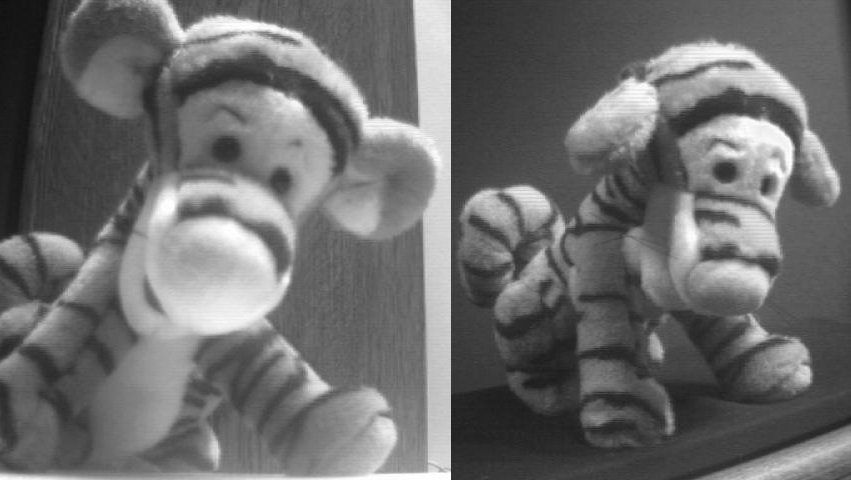
\includegraphics[width=75mm]{figuras/tigger-mit.png}
  \end{center}
  \caption{Brinquedo que responde as emoções das crianças \cite{kirsch1999affective}.}
  \label{fig:tigger-mit}
\end{figure}

O projeto \emph{The Affective Tigger: a reactive expressive toy} de
\citet{kirsch1999affective} é um brinquedo capaz de reconhecer e reagir às
emoções exibidas pelas crianças. Por exemplo, quando a criança encontra-se
feliz, o boneco expressa felicidade (ver Figura~\ref{fig:tigger-mit}). Ao todo
existem 5 estados emocionais: muito feliz, feliz, neutro, triste e muito
triste. Todos, com exceção do neutro, possuem alguma síntese vocal como um
rosnado (tristeza) ou uma risada (muito feliz). Assim, esse brinquedo, por ser
considerado um ser robótico que reage à criança com seus próprios estados
emocionais, fica enquadrado na segunda área.  Portanto, o desenvolvimento
desse brinquedo serviu para aprimorar os seres robóticos.

O projeto AIDA\footnote{Mais detalhes, ver http://senseable.mit.edu/aida} (do
inglês \emph{Affective Intelligent Driving Agent}) pode ser entendido como
enquadrado na área de IHC, pois o interesse é entender o estado afetivo da
pessoa dirigindo. Além disso, interessa-se em ter um relacionamento com o
usuário sugerindo alterações nas rotas baseado na rotina aprendida depois de
um mês de aprendizado.  A pesquisa relatada em \citet{dias-agents} visou
melhorar a simulação de agentes através do uso da emoção guiando o processo
deliberativo e melhorar o entendimento e gerência das emoções.  O presente
trabalho se enquadra na área de síntese de emoção, pois o interesse é em
entender o estado emocional e como ele pode afetar o comportamento de um
personagem.

\section{Modelo Psicológico de Emoção}

Segundo \citet{scherer2000tnoe}, na psicologia há diferentes modelos para
tentar mapear a afetividade: dimensionais, discretos, baseados em significados
e componentes. Os modelos dimensionais procuram estabelecer eixos de classes
de emoções e formas de se mover por esses.  Enquanto os modelos discretos
visam descrever um conjunto básico de emoções ou, ainda, um sistema adaptativo
que evolua a partir de um determinado ponto.  Os modelos baseados em
significados constroem estruturas semânticas e descrevem verbalmente o que
ocorre em determinado sentimento; em outras palavras, preocupa-se com as
situações em que ocasionaram o mesmo. Já os modelos baseados em componentes
entendem que emoções são aprendidas e, sendo assim, estudam o elo entre os
sentimentos e os eventos ou situações que as mesmas acontecem. Esse elo é
montado pela pessoa de diferentes formas.

\citet{Pic98} chama atenção que as emoções sempre foram consideradas um
estigma pela ciência que é fundamentalmente racional com hipóteses testáveis,
argumentos lógicos e experimentos repetitivos.  Entretanto, estudos
neurológicos recentes \cite{ledoux1998emotional,damasio2004erro} mostram a
importância das emoções na tomada de decisão.  \citet{damasio2004erro}
diferencia emoção de sentimento; para ele emoção é um estado físico do corpo e
sentimento é a percepção da mudança desse estado corporal.

\begin{figure*}
  \centering
    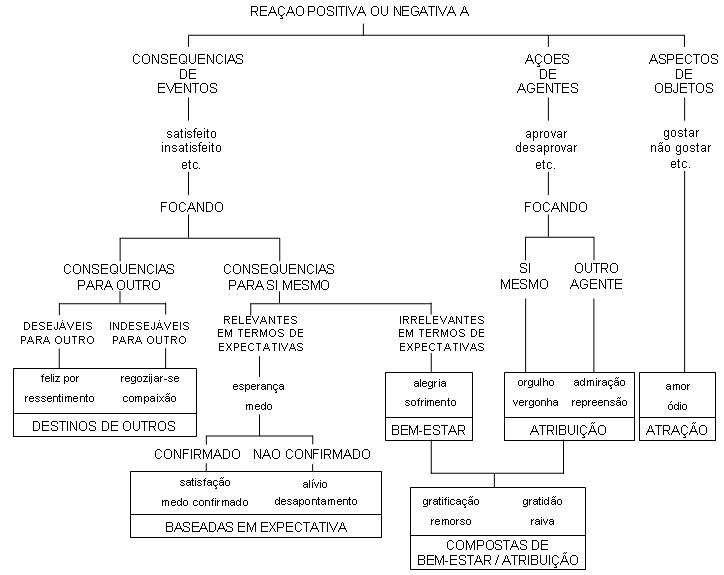
\includegraphics[width=150mm]{figuras/pontarolo_occ.png}
  \caption{Modelo OCC adaptado de \cite{pontarolo2008modelagem}.}
  \label{fig:occ_model_original}
\end{figure*}

O modelo proposto por \citeauthor*{ortony1988cse} \cite{ortony1988cse},
conhecidos na comunidade de Inteligência Artificial, é chamado de OCC por
causa de seus autores.  Esse modelo é classificado como baseado em
significados por descrever as situações de ocorrências de cada uma de suas 22
emoções.  Essas emoções são divididas em formas de se perceber o mundo a sua
volta: Eventos (importantes para alguma meta), Agentes (incluindo a si mesmo)
e Objetos (atração ou repulsa). Assim sendo, essas maneiras de se perceber o
mundo refletem diferentes jeitos de se analisar as situações que podem ser
relativas aos objetivos, valores morais ou gostos da pessoa.

A Figura~\ref{fig:occ_model_original} resume o modelo OCC e mostra as
percepções possíveis de um indivíduo.  Partindo da direita para esquerda, o
ramo mais básico, Aspectos de Objetos, é ativado quando se avalia o gosto de
alguém para algum objeto (inanimado ou não), por exemplo, alguém gostar de
rosas vermelhas.  No seguinte, Ações de agentes, o julgamento das ações
exercidas por outro indivíduo é realizado baseado nos valores morais da pessoa
que está julgando.  Sendo assim, por exemplo, reprovar a atitude de um colega
que ``colou'' na prova. O último da árvore, mais a esquerda, é o de evento que
representa as coisas que aconteceram (e foram consideradas importantes),
acontecem e acontecerão (objetivos almejados). Esses são avaliados segundo as
suas consequências para o alcance ou impedimento dos objetivos de uma pessoa.
Por exemplo, preciso ir bem no concurso para ficar satisfeito porque esse
evento me permitirá alcançar minha meta de ser contratado.

Ainda segundo o modelo OCC, as emoções possuem intensidades. Entretanto, há
distinção entre a valência da emoção e a valência do sentimento. No modelo, um
indivíduo só possui o sentimento quando a intensidade da emoção ultrapassar um
determinado limite.  Essa intensidade é obtida por uma função matemática que
utiliza variáveis de dois tipos: local, que influencia as emoções em um ramo
específico; e global, que influencia todas as emoções do indivíduo.  Um
exemplo de variável local é o desejo, enquanto que um exemplo de variável
global é o senso de realidade.

\section{Ontologias}

\todo{reescrita} Desde Aristóteles, de acordo com \citet{wks2008towards},
começa o estudo das coisas existentes no mundo e a natureza desse existência,
um ramo da filosofia conhecido com ontologia.  Atualmente, na ciência da
computação, ontologias são vistas como um vocabulário de entendimento comum e
compartilhado de um domínio que pode ser utilizada para comunicação entre
pessoas e aplicações distribuídas e heterogêneas.  \citet{ontoly2004Approach}
definem ontologia como uma representação de conhecimento utilizada para
capturar conhecimento e informação sobre determinado assunto, geralmente
estruturado de forma similar a uma rede semântica. Sendo assim, uma ontologia
consiste de um diagrama composto de nodos e arcos que estabelecem uma
fundamentação semântica que permite melhorar a descoberta, interoperabilidade
e reuso do conhecimento.

Logo, o conhecimento pode ser usado de maneiras diferentes e não serve somente
para conter informações em categorias, mas também serve como um tipo de
``banco de dados'' onde instâncias são armazenadas e recuperadas.  O tipo ou
classe da informação possui propriedades que diferem da sua instância. Essa
diferença fica clara quando é feita a comparação da ontologia com uma base de
dados, onde as classes de informações definidas criam as tabelas e as
instâncias povoam os dados nas tabelas.

Na área da computação, ontologias ganharam maior importância com a Web
Semântica permitindo que o conhecimento da página seja facilmente obtido sem
um processamento pesado.  A W3C, orgão internacional que regulamenta padrões
utilizados na Web, regulamentou diversos padrões baseados em \emph{XML} para
ontologias.  A linguagem que será utilizada no presente trabalho será a
OWL\footnote{A sigla vem de ``\emph{Ontology Web Language}''.} e esta fora do
escopo desse artigo aborda-lá em detalhes \footnote{Para mais detalhes, veja
\url{http://www.w3.org/standards/semanticweb/ontology}.}.

\section{Ontologias afetivas}
...

\section{Ontologias de Humanos Virtuais}
...

\section{Trabalhos Relacionados}

O comportamento emotivo do personagem tem um papel importante para se ter a
ilusão de vida conforme afirmou \citet{bates1994role}. Esse trabalho utiliza o
modelo OCC para melhorar a credibilidade dos agentes e cada uma das emoções
pode ser ligada a um comportamento. No exemplo dado anteriormente, um agente
pode ligar o medo a um comportamento agressivo enquanto outro liga essa mesma
emoção de medo a um comportamento de estado alarmado.

\citet{GraCli98} criaram um mecanismo evolucionário utilizando redes neurais
com uma base química para guiar o comportamento do ator. Os atores simulados
podem envelhecer, aprender e, inclusive, se reproduzir (aqui são utilizados
algoritmos genéticos).  Por exemplo, o personagem pode aprender algumas
palavras básicas e demostrar que esta envelhecendo por meio da mudança da cor
de seus cabelos dando uma certa ilusão de vida.

Conforme já dito, as emoções podem melhorar a credibilidade dos seres
virtuais.  \citet{zhang2009emotional} desenvolveram uma aplicação com a
finalidade de demostrar esse conceito. O planejamento das ações a serem
executadas pelo personagem é afetado pelos valores das emoções sendo
experimentadas.

Todos os trabalhos apresentados até aqui, utilizaram as emoções para aumentar
a representação ou expressividade de um ator. Entretanto,
\citet{neto2010construction} tentam estudar o impacto da emoção na decisão dos
agentes.  Assim, para isso ser possível, foi necessário alterar a forma de
planejamento das decisões, além de como recuperar os dados da sua memória.  A
modificação no acesso a memória permite o ``esquecimento'' de determinadas
crenças quando o estado emocional for diferente daquele guardado junto da
memória a ser recuperada. Essa característica torna o planejamento do agente e
as atitudes dos personagens mais realísticas.

\citet{benta2007ontology} e \citet{wks2008towards} descrevem modelos afetivos
através de ontologias. No primeiro trabalho, uma ontologia foi criada
descrevendo emoções primárias e secundárias. O primeiro tipo de emoção exige
menos processamento cognitivo que o segundo. Além disso, o modelo descreve ao
todo 11 emoções sendo 7 dessas consideradas primárias.

 % ou tambem motivacao
%%\chapter{Metodologia}

\section{Atividades previstas}

\begin{enumerate}
	\item Estudo bibliográfico sobre as estratégias existentes de integração de softwares;
	\item Elaboração da proposta de TI e escolha de um segundo orientador (em atendimento à regra do PPGC);
	\item Desenvolvimento da estratégia definida no Jason;
	\item Validação da solução através de ambientes e agentes desenvolvidos em Python;
	\item Redação da monografia;
\end{enumerate}

\section{Cronograma das atividades}

	\begin{tabular}[c]{c|cccccc}
		Atividades & \begin{sideways} \small{Jul/10} \end{sideways}& \begin{sideways} \small{Ag/10} \end{sideways}& \begin{sideways} \small{S/10} \end{sideways}& \begin{sideways} \small{O/10} \end{sideways}& \begin{sideways} \small{N/10} \end{sideways}& \begin{sideways} \small{D/10} \end{sideways} \\ \hline
		%\cellcolor{gray!50} pendente & \\
		%\cellcolor{green!50} feito & \\
		%\cellcolor{blue!50} andamento & \\
		%\cellcolor{red!85} atrasado &  \\
	Estudo bibliográfico & \cellcolor{gray!50} & \cellcolor{gray!50} & \cellcolor{gray!50} &  &  &  \\
	Elaboração proposta &  & \cellcolor{gray!50} &  &  &  &  \\
	Desenvolvimento da estratégia &  &  & \cellcolor{gray!50} &  &  &  \\
	Validação da solução &  & & \cellcolor{gray!50} & \cellcolor{gray!50} &  &   \\
	Redação da monografia &  & \cellcolor{gray!50} & \cellcolor{gray!50} & \cellcolor{gray!50} & \cellcolor{gray!50} &
	\end{tabular}

% Veja modelo em https://saloon.inf.ufrgs.br/twiki-data/PEP/PepEder/pep_v4.pdf
 % nao esquecer o cronograma
%\chapter{Arquitetura Emocional Constru\'ida} \label{ch:aec}

\section{Visão Geral}

A presente arquitetura construída foi pensada conforme mostrado na
Figura~\ref{fig:vasc}. Como se pode observar, o sistema é dividido em um
ambiente e em agentes. O ambiente utiliza as ontologias de preferências e de
rotinas para construir a visualização mostrada no capítulo~\ref{ch:cdu}. Dessa
forma, o que o usuário vê é exibido a partir da descrição da ontologia de
rotinas. Mais detalhes ver seção~\ref{ch:aec:ocu}. Já a de preferências,
explicada na seção~\ref{ch:aec:oda}, permite guardar junto dos objetos do
mundo virtual informações quando as mesmas forem estáticas e criar as
preferências dos agentes sobre essas informações.\dev{}
% O dev colocado acima se deve ao fato de a de preferencias ser guardarem
% informacoes, alem das proprias preferencias.

A segunda parte do sistema altera a mente dos atores agindo para acrescentar
anotações em suas percepções e para alterar local que essas crenças são
salvas. A mente dos atores é chamada agente e eles recebem via percepção as suas
preferências e rotinas\dev{}. Essa escolha foi feita para permitir que a
escolha do que fazer seja toda ela escrita em código\dev{} da plataforma
\emph{Jason}. As emoções são concluídas pelo agente através de ontologia
(ver seção~\ref{ch:aec:omce}) e, portanto, a base de crenças padrão da
plataforma foi estendida para consultar, guardar e recuperar os dados
diretamente nessa quando a crença for relevante. Sendo assim, é como se
houvesse dois níveis. O primeiro formado pela ontologia e o segundo pela base
de crença padrão.

\begin{figure}
  \centering
  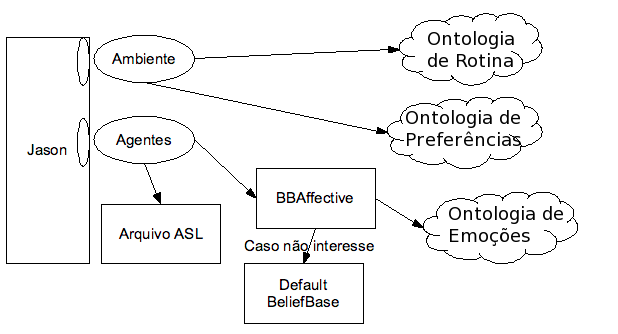
\includegraphics[width=10cm]{figuras/visao-geral.png}
  \caption{Visão abstrata do sistema construído.}
  \label{fig:vasc}
\end{figure}

\section{Ontologia do Modelo Cognitivo Emocional} \label{ch:aec:omce}

A fundamentação do modelo afetivo sendo utilizado aqui é o proposto por
\citet{ortony1988cse} e encontra-se explicado na seção \ref{ch-ca-mce}. A
ontologia proposta tinha como ideia inicial não utilizar regras, porém como
pode ser observado na Tabela~\ref{tab:oa:geral} foi necessário a criação de
regras para suportar o raciocínio no nível de indivíduo corretamente. As
regras que ajudam a conclusão das relações \emph{hasKnow}, \emph{hasFriend} e
\emph{hasEnemy} são diferentes das demais por causa que elas tem como
característica operar no domínio e na imagem da classe \emph{Agent}. Por
exemplo, se John avalia que se relaciona bem com Jose então John
\emph{hasFriend} Jose. Note que o contrario não é necessariamente verdade, o
Jose pode apenas saber que conhece o John então Jose \emph{hasKnow} John.

\begin{table}[h]
	\caption{Ontologia proposta com expressividade: ALCHIN(D).}
	\label{tab:oa:geral}
	\begin{center}
	\begin{tabular}{|c|c|}
	%\begin{tabular}{|p{34mm}|p{50mm}|p{50mm}|}
		\hline
		Descrição & Quantidade \\ \hline
		Classes &  45 		\\ \hline
		Propriedade de Objetos & 16 \\ \hline
		Propriedade de Dados & 14 \\ \hline
		Indivíduos &  0		\\ \hline
		Regras & 7 \\ \hline
	\end{tabular}
	\end{center}
\end{table}

Na Figura~\ref{fig:rlocc} são mostradas as regras desenvolvidas, elas dependem
que os indivíduos da ontologia sejam marcados como diferentes um dos outros.
Assim, recomenda-se fortemente que quando registrar um indivíduo da classe
\emph{Object} ou \emph{Agent} que a informação de igualdade ou diferenciação
seja preenchida\dev{}. Assim, se evita que o raciocinador conclua que não
conhece a resposta e chegue a uma conclusão não esperada.

\begin{figure}[b]
  \centering
  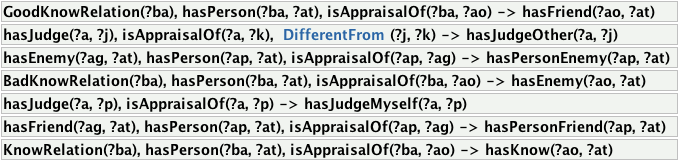
\includegraphics[width=14cm]{figuras/rules-LOCC.png}
  \caption{Regras da ontologia proposta.}
  \label{fig:rlocc}
\end{figure}

A Figura~\ref{fig:kplocc} mostra a árvore de relações que tem como imagem
dados ou instâncias (objetos). Ao se comparar as Figuras~\ref{fig:rlocc}
e \ref{fig:kplocc} se chega a conclusão que as propriedades que as
regras concluem não precisam ser configuradas pelo usuário. Assim, ao invés de
16 propriedades de objetos conforme informado na Tabela~\ref{tab:oa:geral}
apenas 9 precisam ser conhecidas. Dessas, a propriedade menos utilizada é a
\emph{hasSomething} que serve para indicar genericamente o que esta sendo avaliado. Note que
\emph{hasPerson} deve ser usado quando o indivíduo em avaliação for um membro
da classe \emph{Agent}. Já, a relação \emph{hasJudge} serve para indicar que o
membro da classe \emph{Object} esta sendo avaliado pela sua responsabilidade.
Por exemplo, Millie tem uma avaliação julgando seu carro com uma valoração
positiva.

\begin{figure}[b]
  \centering
  \begin{tabular}{cc}
  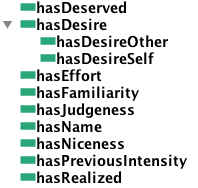
\includegraphics[height=4cm]{figuras/dataProperty-LOCC.png} & 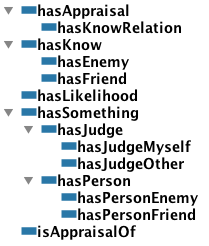
\includegraphics[height=5cm]{figuras/objectProperty-LOCC.png} \\
  (i) Relações de dados & (ii) Relações de Objetos
  \end{tabular}
  \caption{As relações existentes na ontologia proposta.}
  \label{fig:kplocc}
\end{figure}

Todos os dados numéricos da ontologia são inteiros. Isso foi feito com a
finalidade de permitir que o usuário normalize\dev{} o número obtido da
maneira que desejar. Além disso, foi tomada a decisão de não especificar o
domínio da maioria das propriedades por causa que isso forçaria um
enquadramento em classes não desejadas. Por exemplo, se a relação
\emph{hasLikelihood} tiver o domínio \emph{ConsequenceForSelf} e existir um
indivíduo com somente essa relação então o mesmo seria enquadrado no conceito
\emph{ConsequenceForSelf}. Mas, o correto nesse caso seria não ser concluído nada,
ou seja, pertencer à classe \emph{Thing}.

A estrutura da ontologia pode ser visualizada na
Figura~\ref{fig:tlocc}~(pág.~\pageref{fig:tlocc}). Além disso, pode ser
recomendável olhar a
Figura~\ref{fig:occ_model}~(pág.~\pageref{fig:occ_model}) do modelo \occ
durante o resto da discussão dessa seção. Os sub-conceitos de \emph{Emotion}
correspondem aos três ramos do modelo original.
O ramo \emph{ActionsOfAgents} julga a responsabilidade e o quanto o agente que
realizou uma ação ou evento se desviou do esperado, o de
\emph{ConsequencesOfEvents} julga a consequência de um evento e
\emph{AspectsOfObjects} julga a atração para com um objeto.

O primeiro ramo a ser abordado é, o menos cognitivo, \emph{AspectsOfObjects}.
As emoções desse tipo são relacionadas com atratividade e familiaridade.
Entretanto, essas duas relações foram consideradas equivalentes porque o
importante, para o modelo, é quando ambas são positivas ou ambas negativas.
Assim sendo, uma pode assumir os dois papeis sem maiores penalidades e
simplificando a modelagem. A emoção \emph{Hate} é modelada como tendo a
propriedade de familiaridade (\emph{hasFamiliarity}) com valores negativos,
enquanto a emoção \emph{Love} tem valoração dessa mesma propriedade positiva.
Caso o valor seja zero, nada pode ser concluído.

Cabe notar que parece estranho uma emoção \emph{Love} com um objeto, porém
essa emoção foi escolhida por quem montou o modelo para representar seu tipo
por ser a mais forte de sua categoria. Assim, níveis menores implicam em
outros tipos de emoção. Além disso, agentes
podem ser vistos como objetos quando se esta avaliando a sua atração. Logo,
todo agente (\emph{Agent}) é um objeto (\emph{Object}). Por exemplo, John esta
apaixonado pela Millie (\emph{Agent} visto como \emph{Object}) ou John tem
repulsa por televisão.

O segundo conceito, chamado \emph{ActionsOfAgents}, pode ser pensado como
um ramo que julga a responsabilidade por uma determinada ação ou evento.
Assim, esse ramo é capaz de gerar emoções de: Admiração (\emph{Admiration}),
Orgulho (\emph{Pride}), Vergonha (\emph{Shame}) e Reprovação
(\emph{Reproach}). Por exemplo, Jose possui orgulho por cozinhar ou Dilu
reprova Jose porque ele come carne.

Na definição, as emoções de orgulho e vergonha podem acontecer mesmo quando se
esta avaliando ações de outras pessoas. Por exemplo, Dolores tem vergonha de
sua mãe que não cozinha. Essa conclusão é possível por causa de uma relação
que eles propõem de empatia\label{mark:empat}. Entretanto, como em nenhum outro momento, eles
dão mais detalhes sobre essa empatia foi resolvido considerar que vergonha e
orgulho são emoções sentidas somente quando o agente esta avaliando a si mesmo
e, dessa forma, o exemplo anterior não é possível no sistema desenvolvido. \dev{}
% dev -> poderia ter sido usado float e ter feito 1 (para si) e 0 (para outro)

As emoções que julgam responsabilidade são definidas como tendo uma relação de
julgamento (\emph{hasJudge}) e uma relação que mapeia o valor do julgamento
(\emph{hasJudgeness}) que representa o quanto o agente se desviou do
comportamento esperado, isto é, em casos de aprovação é um valor positivo e em
casos de reprovação é um valor negativo. Todavia, isso ainda não permite
diferenciar a emoção de admiração da emoção de orgulho ou a reprovação da de
vergonha. Essa distinção é possível ao se dividir a relação de julgamento com
duas sub-relações: tem auto-julgamento (\emph{hasJudgeMyself}) e tem
julgamento de outro (\emph{hasJudgeOther}).

A utilização de sub-propriedade torna possível escrever a ontologia da maneira
esperada suprimindo o problema. Entretanto, para o usuário pode se tornar
complicado ter que lembrar quando utilizar uma sub-propriedade ou outra.
Assim, foi resolvido deixar o usuário sempre utilizar a relação de julgamento
(\emph{hasJudge}) e via 2 regras inferir se é um auto-julgamento ou o
julgamento de outra pessoa. Para essas regras funcionarem da maneira correta,
o usuário deve declarar que os agentes ou objetos são diferentes uns dos
outros. Caso isso
não ocorra, o sistema considera que não há informação para verificar se um
indivíduo é igual ou diferente e conclui que não conhece a resposta. Além
disso, a relação de julgamento tem como imagem o conceito \emph{Object}. Dessa
forma, os exemplos anteriores são todos válidos.

Cabe salientar que toda avaliação tem pelo menos duas relações. A primeira
relação serve para conhecer quem esta avaliando (\emph{isAppraisalOf}) e a
outra serve para indicar quem ou o que esta sendo avaliado
(\emph{hasSomething}). Essa pode não ser informada explicitamente porque pode
ser concluída quando usada uma de suas sub-relações. O último ramo, chamado de
\emph{ConsequencesOfEvents} é dividido em: \emph{ConsequencesForSelf} e
\emph{ConsequencesForOthers}. Toda essa divisão foca na consequência de um
evento ou ação realizado por algum agente. Por exemplo, Dilu tem pena
de Jose, Jose tem esperança de ser promovido, John tem satisfação por
estar almoçando ou Millie esta alegre por cozinhar.

\begin{wrapfigure}{r}{0.4\textwidth}
  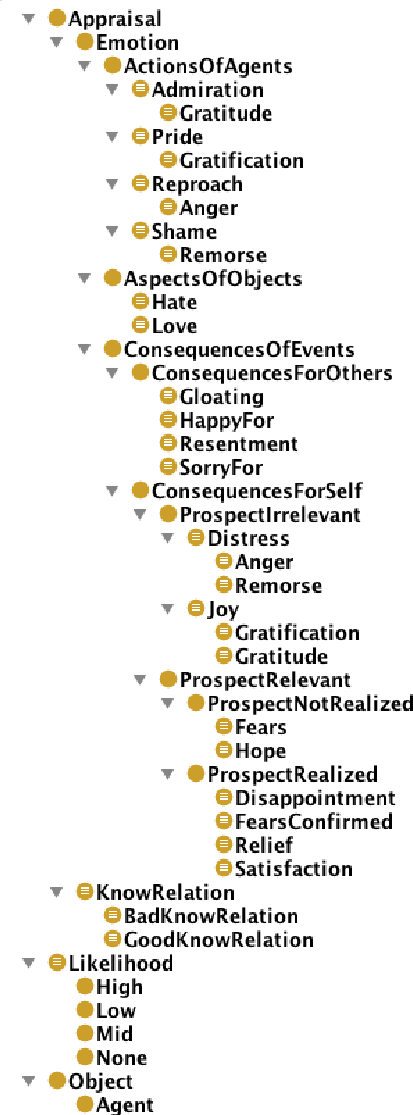
\includegraphics[height=149mm]{figuras/hierarquiaLOCC.png}
  \caption{Taxonomia da ontologia proposta baseado no modelo.}
  \label{fig:tlocc}
\end{wrapfigure}

A \emph{ConsequencesForOthers} expressa 4 emoções: \emph{HappyFor},
\emph{SorryFor}, \emph{Gloating} e \emph{Resentment}. Na definição, essas
emoções dependem: do grau de desejabilidade do avaliador para com o outro; do
grau de desejabilidade que se presume que o outro tenha; do grau de
merecimento do evento; e, do tipo de relacionamento com a pessoa. Na ontologia
proposta, a principal diferença com o modelo \occ é que foi considerado
que o grau de desejabilidade do avaliador para com o outro e o grau de
merecimento do evento são os mesmos. Dessa forma, se pode utilizar apenas três
relações para descrever as 4 emoções.

A relação de merecimento (\emph{hasDeserved}) e de desejabilidade
presumida (\emph{hasDesireOther}) são avaliadas de acordo com sua valoração
positiva ou negativa. A relação \emph{hasPerson} liga o outro indivíduo
sendo avaliado com a avaliação. Para se ter o conhecimento do que esta sendo julgado
ser amigo (\emph{GoodKnowRelation}) ou inimigo (\emph{BadKnowRelation}), esses
conceitos foram criados e precisam ser configurados para cada um dos agentes
em questão. O mesmo pode declarar que só conhece uma pessoa, que conhece e é
um amigo ou que conhece e não gosta dela (inimiga). Entretanto, quem precisa
dessa informação é o conceito de avaliação quando as relações
\emph{hasPersonEnemy} e \emph{hasPersonFriend} precisam ser descobertas.

\emph{ConsequencesForSelf} se divide entre consequências de eventos com
probabilidade relevante (\emph{ProspectRelevant}) e irrelevante
(\emph{ProspectIrrelevant}). Cabe salientar que esses dois conceitos se
relacionam com probabilidade (\emph{hasLikelihood}), entretanto enquanto o
primeiro conceito se relaciona com a parte não nula. A outra se relaciona
somente com essa. Dessa forma, ambos os conceitos são disjuntos. A classe de
probabilidade relevante pode ser dividida ainda entre possibilidade não
realizada (\emph{ProspectNotRealized}) e realizada (\emph{ProspectRealized}).

As emoções \emph{Hope} e \emph{Fear} fazem parte do conceito
\emph{ProspectNotRealized}. Esse conceito usa as relações \emph{hasLikelihood}
e \emph{hasDesireSelf}. Essa última é um número que
representa o desejo de se obter ou repudiar o evento. Além disso, quando o
evento ocorre a emoção atual pode virar uma emoção do conceito
\emph{ProspectRealized}, isto é, \emph{Fear} pode virar ou
\emph{FearsConfirmed} ou \emph{Relief} e \emph{Hope} pode virar ou
\emph{Satisfaction} ou \emph{Disappointment}.

O conceito \emph{ProspectRealized} não se relaciona em nenhum momento com a
relação \emph{hasLikelihood} porque o evento já aconteceu ou não vai mais
acontecer. Assim, ele possui três relações distintas das anteriores, a
primeira é o grau de realização de um evento (\emph{hasRealized}), isto é, a
visão do agente sobre como a consequência do evento aconteceu. A segunda
relação \emph{hasPreviousIntensity} recebe a valoração da emoção de medo ou
esperança do evento que tinha probabilidade e serve para saber se o evento era
um evento bom (esperança) ou ruim (medo). Já, a terceira \emph{hasEffort}
tenta estimar o grau de esforço que foi dispendido para a atração ou repulsa
da consequência do evento.

O conceito \emph{ProspectIrrelevant} é parecido com o conceito
\emph{ProspectRelevant} com a diferença que a relação \emph{hasLikelihood} vai
somente para valores nulos. Fora isso, as emoções desse conceito e do
\emph{ActionsOfAgents} podem ser misturadas formando conceitos compostos.
A composição é quando uma emoção pode ser encaixada em mais de uma emoção
como no caso de se estar alegre (\emph{Joy}), orgulhoso (\emph{Pride}) e
gratificado (\emph{Gratification}). Por fim, o conceito \emph{Setup}
é o utilizado para manter junto da ontologia criada o limite mínimo para uma
emoção virar sentimento\dev{}.

%a transferencia eh feita pelo sistema;
%os dados sao carregados para memoria e eliminados;
%conforme reparado nao ha decaimento da emocao, a mesma eh instantanea;
%2345678901234567890123456789012345678901234567890123456789012345678901234567890

\section{Ontologia de Comportamento Urbano} \label{ch:aec:ocu}

O presente trabalho foca no comportamento de personagens. Dessa forma, uma
ontologia de comportamento urbano tenta descrever a vida normal que um
personagem leva. De outro modo, isso pode ser visto como a rotina regular que
o ator possui em sua cidade virtual.

\begin{figure}
  \centering
    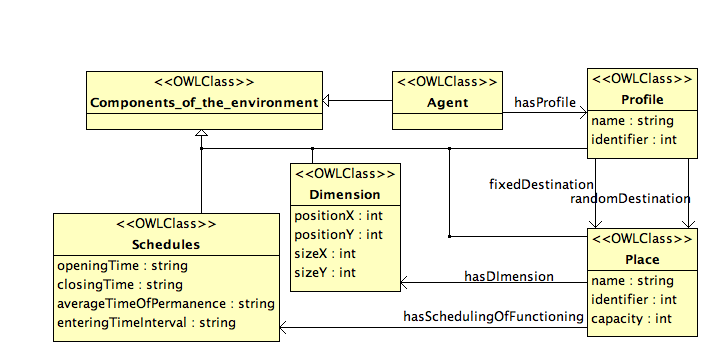
\includegraphics[width=150mm]{figuras/uem-tbox.png}
  \caption[T-Box baseado no modelo de ambiente urbano.]{T-Box baseado no modelo de ambiente urbano \cite{paiva2005ontology}.}
  \label{fig:UEM:TBOX}
\end{figure}

A Figura~\ref{fig:UEM:TBOX} demostra a ontologia, criada por
\citet{paiva2005ontology}, que será utilizada. As relações de generalização
possuem a mesma semântica que na UML, as relações direcionais são relações
binárias entre as instâncias das classes. Na figura, \emph{Agent} se relaciona
com o conceito \emph{Profile} para determinar o tipo de agente. O
\emph{Profile} do agente pode variar entre alguns tipos especificados pelo
usuário que podem possuir destinos fixos (usuais) ou destinos randômicos
(eventuais).

Esses locais são definidos pelo conceito \emph{Place} que contêm
uma descrição de sua capacidade (quantidade máxima de atores), dimensão
(acessível por relação) e horário de funcionamento (acessível por relação). O
conceito de \emph{Dimension} guarda a posição e o tamanho nos eixos X e Y. Já,
o conceito de \emph{Schedules} possui o horário de abertura e fechamento,
intervalo de entrada e tempo médio de permanência.

Além disso, o conceito \emph{Components\_of\_the\_environments} esta sendo
pensando como um sub-conceito de \emph{Setup} na ontologia
desenvolvida por causa que esse representa as configurações gerais.
%
%Essas configurações gerais são carregadas, normalmente, em outras partes do
%sistemas e então eliminadas por causa que elas não influenciam as emoções
%diretamente.
Fora isso, foi introduzido uma nova relação chamada \emph{hasCharacter} que
mapeia o conceito de agente da ontologia anterior para o conceito apresentado aqui.
Dessa forma, um agente na ontologia afetiva pode descobrir seu perfil e descobrir seus locais visitados
regularmente. O conceito de \emph{Place} pode ser pensado, como veremos
adiante, como um ``objeto inteligente''.

Essa ontologia é utilizada no presente trabalho de duas formas. A primeira
forma de utilização é para desenhar um mapa 2D do ambiente que os agentes
atuam. Isso é permitido porque o conceito \emph{Place} relaciona-se com o
\emph{Dimension}. Assim, todos os itens do mapa são retângulos. A outra forma
de utilização é a que trouxe a ontologia para o trabalho e é definir que um
agente tenha sua rotina descrita e disponibilizada pelo ambiente. Para o
ambiente disponibiliza-la via percepção, no ambiente simulado construído cada
dia simulado equivale a aproximadamente 96 ciclos. Isso quer dizer que cada
passo simulado seria em torno de 15 minutos de um dia. Dessa forma, o ambiente
é responsável por conhecer que dia é e informar cada agente de sua rotina para
aquele dia simulado.

\section{Ontologia de Preferências} \label{ch:aec:oda}

\citet{doyle1998annotated} propuseram que o mundo contivesse uma série de
anotações nos objetos. Assim, o agente poderia conhecer apenas a forma de
questionar os objetos sobre suas formas de usar, suas descrições e suas outras
características. Esse conceito veio do conceito \emph{affordance} que se
refere a propriedade de um objeto que dita como o mesmo será utilizado.
Dessa forma, uma cadeira tem a propriedade de ser sentada e uma porta tem as
propriedades de ser aberta ou ser fechada.

Assim, eles utilizaram 5 tipos de anotações: (i) anotações emocionais,
explicam como um agente responde ``emocionalmente''; (ii) anotações de
resposta, explicam como o agente deve reagir ao evento no ambiente que pode ser
uma ação especifica ou uma sugestão de crença; (iii) anotações de resolução de
problemas, descreve o estado do problema e permite anotar dicas que o ator
talvez fale ou realize; (iv) anotações de papel, informam o agente sobre ações
relevantes para determinados trabalhos no mundo; (v) anotações de jogo,
descrevem o estado do jogo permitindo sugerir movimentos.

\citet{kallmann1999modeling} explicaram uma ideia similar, os objetos no mundo
são os responsáveis por proverem para o personagem o como ele deve ser usado.
Por exemplo, durante a animação do personagem estar abrindo uma porta, quem esta
no controle do ator é o ``agente'' que controla a porta. O agente do
personagem delega a responsabilidade da animação para o agente do objeto por
causa que o mesmo é o único que sabe como realizar a animação de abertura ou
fechamento da porta. Esses objetos, denominados objetos inteligentes, precisam
ter um determinado nível de conhecimento sobre o personagem.

De uma maneira similar, o conceito de artefatos que possuem propriedades
observáveis e utilizáveis foi criado por \citet{ricci31cartago}. Por exemplo,
uma porta pode ter como propriedade observável seu estado (estar aberta ou
estar fechada) e ação possível ou propriedade utilizável ser aberta ou ser
fechada. Essas ações podem ficar disponíveis conforme o estado atual do
objeto, mas o controle da disponibilidade e da ação é do próprio objeto por
que é ele que sabe como realizar a ação propriamente dita. O agente unicamente
diz de alguma forma que o objeto tem que realizar tal ação. Nesse trabalho,
não é mencionado que o agente pode ser temporariamente controlado por
objetos.

\begin{figure}
  \centering
    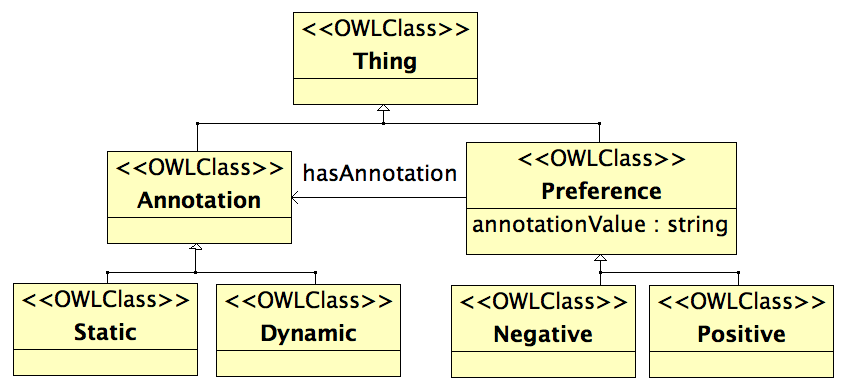
\includegraphics[width=130mm]{figuras/preferences.png}
  \caption{T-Box da ontologia de preferências proposta.}
  \label{fig:preferences}
\end{figure}

A ontologia proposta para as preferências pode ser vista na
Figura~\ref{fig:preferences}. Como pode ser observado, foi criado dois
conceitos principais \emph{Annotation} e \emph{Preference}. O conceito
\emph{Annotation} é utilizado para representar características de determinadas
coisas. Essas características podem ainda ser categorizadas entre as que mudam
e não mudam durante a simulação. O sub-conceito \emph{Dynamic} representa as
características dinâmicas, isto é, as características que podem ser alteradas
durante a ``vida'' do objeto. O sub-conceito \emph{Static} representa as
características que não podem ser alteradas depois da criação do objeto. O
calor e o dono são exemplos de características dinâmicas, enquanto o nome e a
capacidade total são exemplos de características estáticas.

O conceito \emph{Preference} é usado para representar as preferências por
determinadas características ou anotações. A preferência define como uma entidade ou
agente é atraído por determinada característica, por exemplo algumas pessoas
gostam de calor e outras não. Assim, as pessoas que gostam de calor são
atraídas pela valoração positiva da anotação de calor. Já, as pessoas que não
gostam de calor são atraídas pela valoração negativa. Dessa forma, os
sub-conceitos da preferência representam sempre valores que fazem o agente ser
atraído pelo objeto e repelido caso contrário.

Entretanto, esse exemplo não funciona para todos os casos. Por exemplo, um
agente tem conhecimento de seu nível de energia e este é sempre positivo. Para
resolver esse problema foi criada a relação \emph{hasAnnotationValue}
representada na Figura~\ref{fig:preferences} pelo atributo
\emph{annotationValue}. Sendo assim, é possível descrever que um agente com
nível de energia abaixo de um determinado limite é atraído pelo seu centro de
controle.

Essas anotações foram planejadas para serem colocadas pelo ambiente
nos objetos e nos agentes. As anotações em agentes permitem que os outros saibam
o que o agente esta fazendo e como ele parece de forma similar aos objetos. As
preferências também são disponibilizadas em formas de percepção, mas o usuário
que deve criar regras ou planos no \jason para montar as relações usadas pela
afetividade.

\section{Integrando a Plataforma \jason com as ontologias} \label{ch:p:ipjo}

As ontologias explicadas, nas seções anteriores, foram planejadas para serem
usadas como módulos. Sendo assim, as ontologias explicadas anteriormente
podem ser usada sem implicar no uso das demais. Cabe salientar que elas podem ser
usadas tanto pelo agente quanto pelo ambiente conforme poderá ser visto no
capítulo~~\ref{ch:cdu}.

\begin{figure}[b]
  \centering
  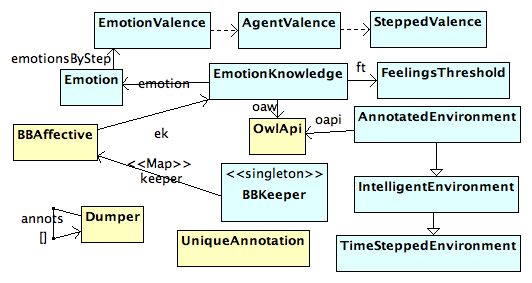
\includegraphics[width=8cm]{figuras/implementacao-15dez2011.png}
  \caption{Diagrama de classes do sistema.}
  \label{fig:dcs}
\end{figure}

Na figura~\ref{fig:dcs} pode ser observado as classes desenvolvidas para
realizar a integração das ontologias com os agentes \jason e o suporte
afetivo. Para essas classes
serem usadas, o agente deve ser configurado para utilizar a classe
\emph{BBAffective} como base de crença. Essas para a implementação da
afetividade funcionar perfeitamente. Essa configuração pode ser feita conforme explicado na
seção~\ref{sec-jason-architecture} (pág.~\pageref{sec-jason-architecture}) e
demostrado na seção~\ref{ch:cdu:tbc} (pág.~\pageref{ch:cdu:tbc}). A classe
\emph{UniqueAnnotation} é a responsável por garantir a não duplicidade de
anotações. %Assim,
%quando se insere por algum motivo duas vezes a mesma anotação apenas valerá a
%última.

A responsabilidade da classe \emph{BBAffective} é manter as crenças dos
agentes e atender as solicitações da plataforma \jason sobre a manipulação
dessas em dois níveis. O primeiro nível é a ontologia e o segundo é a base de
crença padrão que é utilizada quando o elemento não é considerado relevante
para o primeiro nível. A relevância é descoberta consultando os conceitos e
propriedades existentes na ontologia, por exemplo instâncias de conceitos são
crenças no formato ``nomeDoConceito(nomeDaInstancia)'' e relações são
similares à ``nomeDaRelacao(nomeDaInstanciaDominio, Imagem)''. Conhecer o que
é relevante para a ontologia é necessário porque a mesma é lenta e quanto
menos elementos contiver nela melhor será seu desempenho.

A base de crenças delega todo o assunto relacionado com as crenças da
ontologia para a classe \emph{EmotionKnowledge}. Essa é responsável por
conhecer todo o assunto relacionado com as emoções e sentimentos, porém ela
delega o conhecimento da história da potência das emoções para a classe
\emph{Emotion} e o conhecimento dos limites de ativação para a
\emph{FeelingsThreshold}. Da mesma forma, a manipulação e consulta da
ontologia, propriamente dita, é de responsabilidade da classe \emph{OwlApi}.

A classe \emph{Emotion} é responsável por conhecer todas as emoções presentes
e seus valores de potência. Para isso, no inicio da simulação a ontologia é
consultada procurando por todas as classes definidas\footnote{As classes
definidas possuem condições necessárias e suficientes, isto é, qualquer
indivíduo pode ser enquadrado nessa classe desde que obedeça as condições
suficientes.} sobre o conceito ``Emotion''. Isso é utilizado pela classe
\emph{EmotionKnowledge} quando a mesma precisa consultar o nome de uma emoção
por algum motivo. Por exemplo, na hora de calcular a valência da emoção em um
determinado passo é pedido pelo nome de todas as emoções à essa classe. Essa
ainda mantém a história da potência das emoções por agente para cada ciclo
armazenado utilizando um objeto da classe \emph{EmotionValence} que é um
extensão da classe \emph{HashMap} do \emph{Java}.

Para o suporte emotivo funcionar, a classe \emph{FeelingsThreshold} precisa
retornar que todos os limites mínimos de sentimentos estão configurados.
Assim, ela é responsável por fazer essa verificação e por disponibilizar esses
limites para quando for realizado o cálculo da valência. Esse cálculo é
coordenado pela \emph{EmotionKnowledge} que consulta a ontologia, via instância
da classe \emph{OwlApi}, procurando os indivíduos do conceito ``Appraisal''
visando obter as relações de dados desses indivíduos. Dessa forma, a potência
é a soma de todas as propriedades numéricas de um mesmo indivíduo.

As classes de ambiente, isto é, as classes que possuem \emph{Environment} no
nome são responsáveis por diversas coisas relacionadas com o mesmo. Por
exemplo, manter os passos de simulação com um tempo máximo, conhecer a
quantidade de agentes que tem que esperar responderem para ir ao passo de
simulação seguinte, carregar as ações definidas pelo usuário a partir de um
determinado pacote especificado e etc. Cabe salientar, as ações definidas no
ambiente precisam estender a classe \emph{EnvironmentAction} (não desenhada) e
estarem no pacote especificado na chamada a função ``loadAllActions''.

A classe \emph{Dumper} é responsável por conhecer o formato das crenças \jason
e converte-lo para um formato interno. Isso é necessário para proteger o
código feito de mudanças que a plataforma venha a ter. Assim, essa classe é
utilizada por todas as classes internas do sistema e, principalmente, pela
\emph{BBAffective} após constatada a relevância do elemento. Algumas funções
desse tipo são devolver os parâmetros do literal como \emph{string} ou número,
retornar uma instância de seu tipo a partir de um literal, criar o literal a
partir de uma \emph{string} ou a partir de uma outra instância de seu tipo e,
até mesmo, realizar a criação de um \emph{XML} para transferir os dados para
à ontologia.

Já, a classe \emph{BBKeeper} serve para facilitar o acesso a base de crenças.
Essa classe é a única \emph{singleton} do sistema e cada instância da
\emph{BBAffective} é conhecida por esta a partir do nome de seu respectivo
agente. Isso é muito útil para os exemplos porque torna possível acessar a
base de crenças e exibir os valores de potência e valência ou conhecer os
tipos emotivos disponíveis. Cabe salientar que os tipos emotivos disponíveis
do simulador não levam em conta o agente e, por isso, mesmo que seja usado um
agente que não esteja utilizando a base estendida os tipos serão retornados
corretamente.

As seções seguintes, explicam os novos processos de inserção, remoção,
consulta e listagem das crenças. Exemplos desses em código \jason são,
respectivamente, \emph{+crencca}, \emph{-crencca}, \emph{?crencca} e
\emph{?X}. A listagem, também, é utilizada pela tela de visualização de
crenças quando se esta realizando uma depuração no agente.

\subsection{Processo de Listagem e Consulta de Crenças}

\begin{figure}
  \centering
  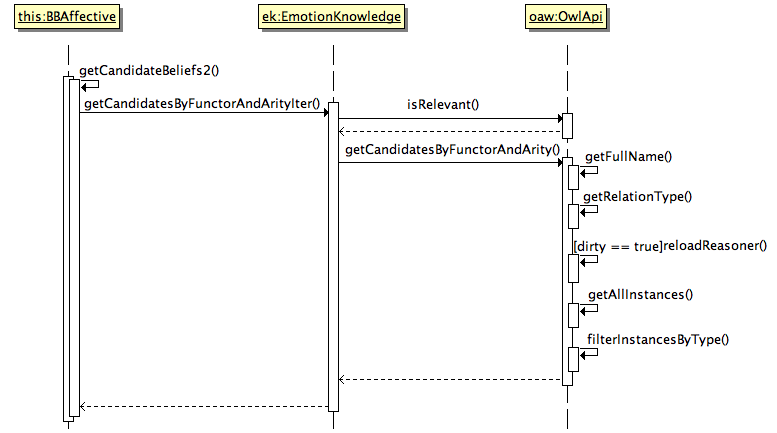
\includegraphics[width=12cm]{figuras/sd-getCB.png}
  \caption{Diagrama de sequência para consultar uma crença.}
  \label{fig:getCandidates}
\end{figure}

O processo de listagem serve para exibir todas as crenças e percepções do
agente. Isso é importante em momentos de depuração ou em momentos que se
deseja consultar uma crença que é uma variável não unificada, isto é, sem
valor definido. Dessa forma, a base de crenças implementa a interface
\emph{java.lang.Iterable} que permite a classe ser usada em construções
\emph{for-each}. A implementação devolve todos os elementos dos dois níveis
sendo que o nível da ontologia é recuperado primeiro.

De maneira similar, o processo de consulta de crenças foi alterado.
%Entretanto, ele pode ser chamado via código \jason ou pelo código \emph{Java}.
Esse processo tem como entrada os métodos com nome \emph{getCandidateBeliefs}
que chamam um método comum denominado \emph{getCandidateBeliefs2} conforme
pode ser visto na Figura~\ref{fig:getCandidates}. O resultado dessa operação é
um objeto \emph{Iterator} com todas as crenças recuperadas da base que possuem
o mesmo nome e mesma aridade que a informada na chamada. Isso é importante
porque esses candidatos podem ter seus parâmetros verificados pela própria
base de crenças ou por outros pontos de acesso do \emph{Jason}.

\subsection{Processo de Recuperação de Crenças}

O processo de recuperação de uma crença é necessário para o entendimento das
inserções e remoções de crenças. Ele serve para recuperar uma única crença
quando ela já existir na base. Esse processo leva em consideração toda a
estrutura do literal, desconsiderando somente as anotações do mesmo em suas
buscas.

A Figura~\ref{fig:recover} mostra esse processo de recuperação. Ele inicia com
a chamada à \emph{getCandidateBeliefs} que foi explicada na seção anterior.
Cada um dos candidatos retornados pela chamada são verificados para ver se
conferem com o informado pelo cliente, se conferir então o candidato é
retornado. Se nenhum candidato for retornado, o resultado da base de crenças
padrão será retornado porque o mesmo pode estar localizado neste nível.
Conforme foi falado anteriormente, tanto a inserção e remoção utilizam esse
procedimento para recuperar o elemento armazenado na base de crença, porém os
motivos serão vistos em suas respectivas seções.

\begin{figure}
  \centering
  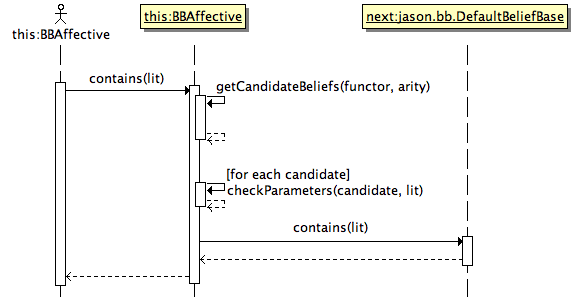
\includegraphics[width=100mm]{figuras/sd-contains.png}
  \caption{Diagrama de sequência para recuperar uma crença.}
  \label{fig:recover}
\end{figure}

\subsection{Processo de Adição de Crenças}

O procedimento de inserção de uma crença pode ser visto na
figura~\ref{fig:addBelief}. Essa figura utiliza as guardas do UML que são
etiquetas com o texto entre colchetes para informar a condição que o código
deve ter para ser executa. Além disso, elas encontram-se localizadas perto de
um quadrado para simbolizar que todas as chamadas feitas dentro deste estão
relacionadas aquelas condições. Dessa forma, quando estiver sendo inserida uma
crença de percepção com o termo diferente de ``step'' nenhum código será
executado pelo diagrama e a mesma será inserida no segundo nível.

A chamada do \jason para a função \emph{add} não se encontra representada na
figura~\ref{fig:addBelief}, porém essa função chama uma outra de mesmo nome e
quando essa retorna falso é chamada a função \emph{add} da instância
\emph{next}. Cabe chamar atenção que quando uma percepção esta sendo inserida
e o termo da crença é ``step'' é realizado o processo de sumarização que
calcula e guarda a potência da emoção na classe \emph{Emotion}. Além disso, se
aproveita o momento para obter e inserir na base de crenças padrão os
sentimentos que acabaram de sofrer atualização em seus valores.

\begin{figure}
  \centering
  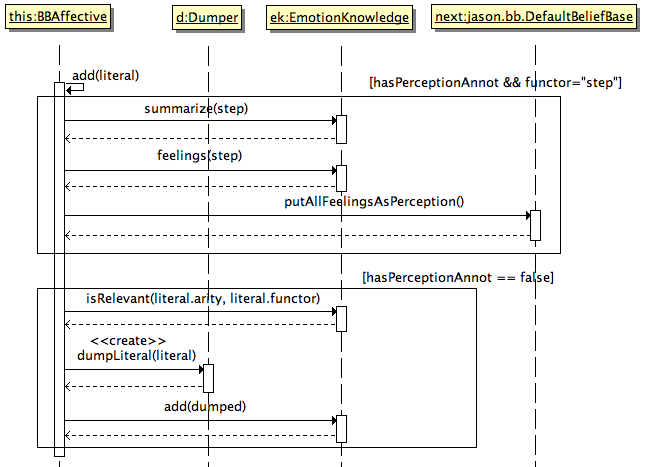
\includegraphics[width=12cm]{figuras/addB.png}
  \caption{Diagrama de sequência para adicionar uma crença.}
  \label{fig:addBelief}
\end{figure}

Agora quando esta sendo feita uma inserção de uma crença que não é uma
percepção, é feita a verificação se ele é relevante. Caso ele seja considerado
irrelevante, a crença sera inserida no segundo nível. Entretanto, se ele for
considerado relevante então será feita a recuperação do elemento atualmente
armazenado e, após isso, é feita a inserção das novas anotações nesse
elemento. Se o elemento não existir na base de crenças então esse último
procedimento é ignorado, porém ele é necessário para haver a correta
atualização das anotações. Por fim, a crença é transformada no tipo interno e
enviado para ser acrescentado na ontologia.

Assim, o processo de inserção serve para inserir os axiomas necessários para
representar essa crença na ontologia quando a mesma for relevante. Para a
criação na ontologia, é necessário ainda diferenciar se é uma instância de
objeto ou propriedade de dados ou de objetos. Essa diferenciação é feita pela
aridade e, em caso de ambiguidade, se pergunta o tipo à ontologia usando o
nome da entidade.

\subsection{Processo de Remoção de Crenças}

O processo de remoção de crenças permite remover uma crença da base de crenças
ou, apenas, atualiza-la retirando alguma anotação que não devia existir. Dessa
forma, o procedimento ao final do mesmo remove os axiomas postos anteriormente
e os insere novamente quando for uma atualização. A Figura~\ref{fig:delBelief}
mostra a rotina da base de crenças.

\begin{figure}
  \centering
  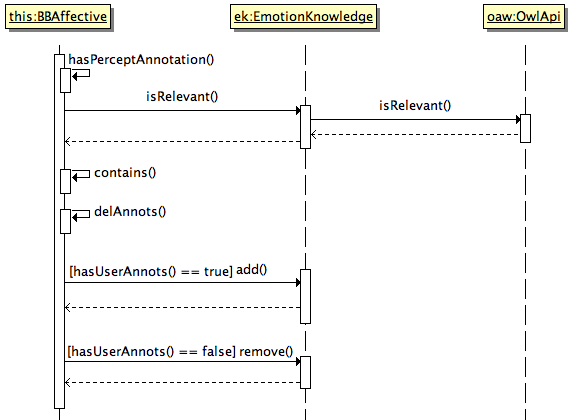
\includegraphics[width=10cm]{figuras/delB.png}
  \caption{Diagrama de sequência para remover uma crença.}
  \label{fig:delBelief}
\end{figure}

A rotina de remoção desenvolvida, inicia verificando se o termo pode ser
considerado relevante. Se ele for uma percepção então ele é irrelevante para
esse procedimento. Caso não seja uma percepção, a relevância é verificada e
se for relevante então é recuperado o elemento armazenado. Se não for
recuperado nenhum elemento ou se ele for irrelevante então é realizada a
chamada a remoção da base de crenças padrão e retornado o resultado.

Nesse momento que se sabe a crença armazenada pelo agente e que a mesma
é relevante. As anotações informadas são removidas da crença obtida e a nova
crença é testada para ver se ainda possui anotações. Se possuir e não for uma
anotação de fonte e não é um indicativo de estar sendo armazenada em
determinada ontologia então é feita a atualização do valor armazenado. No caso
de não possuir anotação ou possuir somente as anotações anteriores mencionadas
é feita a remoção do elemento.

\subsection{Processo Compartilhado de Remoção e Adição de Crenças}

O processo de adição e remoção de crenças compartilham pedaços de códigos. A
classe \emph{EmotionKnowledge} possui dois pontos de entrada, um pelo método
\emph{add} e outro pelo método \emph{remove} tanto um quanto outro fazem uma
chamada para uma função denominada \emph{changeBelief} informando esta se é um
procedimento de inserção ou remoção. A partir dai a sequência de chamadas
mostradas na Figura~\ref{fig:shareBelief} segue de maneira igual. Isso foi
feito porque muito código é igual tanto para um quanto para outra parte.

\begin{figure}
  \centering
  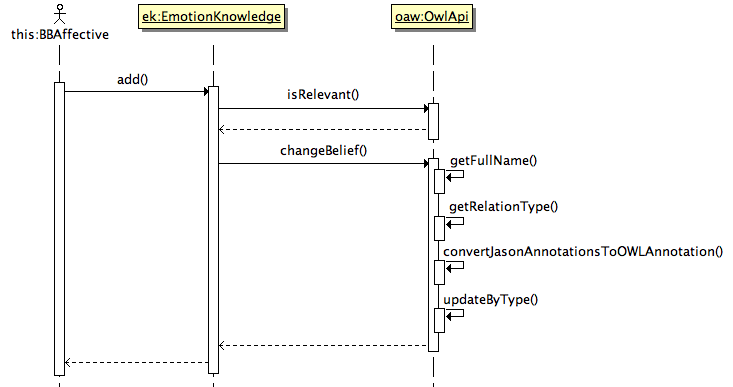
\includegraphics[width=12cm]{figuras/shareBelief.png}
  \caption{Diagrama de sequência para adicionar uma crença.}
  \label{fig:shareBelief}
\end{figure}

A classe \emph{OwlApi} é a única que consulta a ontologia diretamente via
biblioteca. No inicio da aplicação são extraídas as informações de quais
conceitos existem, quais relações e de que tipos elas são. Sendo assim,
consultar o nome completo de uma determinada entidade ou qual é seu tipo não
precisa ir na ontologia. A função \emph{updateByType} é a responsável por
realizar a inserção e remoção das entidades. Uma alteração é feita removendo
a entidade anterior e acrescentando uma nova e marcando a ontologia como suja
para quando uma consulta for feita a mesma ter o raciocinador atualizado.


%%\include{objetivos} % e resultados esperados
%\chapter{Considerações finais}

O presente artigo visa apresentar uma visão do trabalho que está sendo feito
para a construção de um simulador no qual os atores e ambientes interagem.
Entretanto, a ontologia foi omitida porque está ainda sendo aprimorada.  A
idéia apresentada não é nova, porém, o ponto chave é a ontologia permitir aos
agentes raciocinarem sobre suas emoções de forma transparente.  Essa
transparência é útil porque permite ao animador conhecer e, até mesmo,
especificar o personagem com um grau bastante elevado de abstração.
%
Dessa forma, dois agentes com a mesma especificação, ao enfrentarem a mesma
situação, terão o mesmo comportamento quando tiverem vivenciado as mesmas
experiências. Essa experiência inclui as informações adquiridas sobre o
ambiente e sobre os demais atores e não somente os interesses e metas do
mesmo.

O modelo OCC em uso no presente trabalho, foi definido em
\citeyear{ortony1988cse} e possui ao todo 22 emoções especificadas por regras
que demonstram quando a mesma acontece. Entretanto, em nenhum momento da sua
definição foi tratado explicitamente como uma emoção afeta as outras presentes
no personagem.
%
A ferramenta em desenvolvimento tem como interesse a simulação computacional
do comportamento humano e, dessa forma, ela pode ser utilizada de diferentes
maneiras e pode coletar diferentes informações para análises com diversos
propósitos.

%% TODO: versoa anterior fim
\chapter{Introdução}

Ontologia foi caracterizada como o estudo da existência, desde Aristóteles,
por estar interessada em descrever todas as coisas existentes e as relações
que existem entre elas. Atualmente, essa forma de representar o domínio do
conhecimento tem se tornado popular na computação por causa da independência
de sistema oferecida.

Segundo \citet{gruber1993translation}, uma ontologia é uma especificação explícita do
domínio sendo tratado. Além disso, ele aplica esse conceito em sistemas
baseados em conhecimento onde o domínio é representado por um formalismo
declarativo e o conjunto de conceitos e relações forma o vocabulário usado
pelo sistema. Esse vocabulário provém um conjunto de termos bem formados para
o sistema trabalhar.
%
Entretanto \citet{ontoly2004Approach}, definiu ontologia como uma representação
do conhecimento usado para capturar outras informações ou conhecimentos sobre
o assunto. Atualmente, ontologias são vistas como um entendimento comum e
compartilhado de um domínio que pode ser utilizado na comunicação entre
máquinas ou entre pessoas \cite{wks2008towards}.

O presente trabalho foi baseado na linguagem OWL (\emph{Ontology Web
Language}). Essa linguagem foi regulamentada pela W3C\footnote{Ver
\url{http://www.w3.org/standards/semanticweb/ontology}.}, orgão internacional
que regulamenta padrões na Web, para ser usada na \emph{Web} Semântica.
Essa linguagem foi criada em 2002 com o proposito de criação de ontologias e
trabalha com a hipótese de mundo aberto, isto é, nada é afirmado por não ser
dito. Infelizmente, para a W3C não há uma distinção clara entre vocabulário e
ontologia.

A linguagem OWL permite a especificação de conceitos e não de suas instâncias.
Sendo assim, não é possivel descrever uma regra simples como um conceito de
igualdade onde duas relações distintas tem que chegar na mesma instância
final. %Outro exemplo, o conceito de tios que são os irmãos de meus pais não é
%possível ser feita na OWL. A versão 2 da OWL permite a descrição do conceito
%de tios, porém o conceito de igualdade permanece impossível.
%
A linguagem SWRL (\emph{Semantic Web Rule
Language})\footnote{Mais detalhes \url{http://www.w3.org/Submission/SWRL/}.}
recomendada pela W3C permite escrever regras lógicas que melhoram a
precisão dos conceitos sendo descritos porque permite lidar com as suas
instâncias. Dessa forma, a SWRL supri uma falta até então não tratada pela
linguagem OWL e, por isso, seu uso em conjunto é extremamente poderoso. Essas
duas linguagens juntas permitem a escrita do conceito de igualdade descrito
anteriormente.

A ferramenta \emph{Protege}\footnote{Mais informações, consulte \url{http://protege.stanford.edu}.}
em sua versão 4.1 suporta a linguagem OWL 2 juntamente com a SWRL. Ha suporte
aos raciocinadores chamados \emph{FaCT++}, \emph{HermiT} e \emph{Pellet}.
O raciocinador é uma peça importante porque é através dele que a ontologia
será questionada, isto é, somente com um raciocinador ativo é possível saber
se uma instância pertence a determinado conceito. O raciocinador
\emph{Pellet}\dev{} é o que esta sendo utilizado pelo presente autor por
seu excelente suporte a explicações de inconsistência.

A área da computação que estuda as emoções é denominada Computação Afetiva por
\citet{Pic98}. As emoções, segundo \citet{damasio2004erro}, podem ser divididas
entre primárias (não-cognitivas) e secundárias (cognitivas). As emoções
primárias surgem a partir de reações a determinados estímulos e são geradas
rapidamente. Já as emoções secundárias são aprendidas ao longo da nossa vida,
isto é, são geradas por uma avaliação de uma situação de acordo com nossos
objetivos e valores morais. Entretanto, essa divisão ainda não esta
consolidada porque o fato de haver menos atividade cognitiva não quer dizer
que esta atividade não exista.

\citet{bates1994role} foi um dos primeiros a trabalhar na utilização de
emoções na área de animação. Nessa área, o estudo do comportamento humano é
realizado visando realizar a imitação das ações humanas. Assim, simulando
essas atitudes de uma pessoa de tal maneira que pareça possuir vida própria.
Seu trabalho utilizou o modelo de emoções proposto por \citet{ortony1988cse}.
Esse modelo fundamenta ao todo 22 emoções diferentes divididos em três
formas de percepção: ações, eventos e objetos.

%\begin{figure*}
%  \centering
%    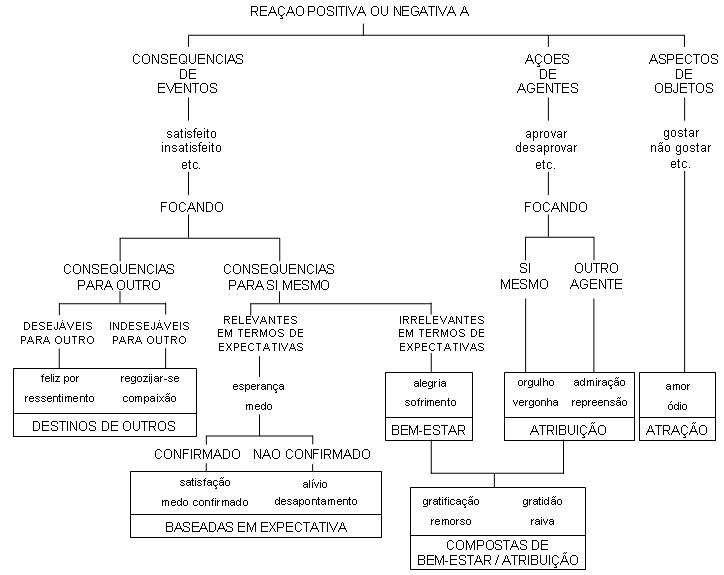
\includegraphics[width=100mm]{figuras/pontarolo_occ.png}
%  \caption{Modelo OCC adaptado de \cite{pontarolo2008modelagem}.}
%  \label{fig:occ_model_original}
%\end{figure*}

A Figura~X\footnote{removido por agora} mostra uma visualização da estrutura
lógica das emoções. As emoções no modelo de \citet{ortony1988cse} já
encontram-se agrupadas em grupos por estarem utilizando regras semelhantes ou
próximas. Esses grupos são representados pelo quadrados e nome do grupo é dado
na parte inferior, assim o ramo de objetos que julga a atração de um indivíduo
com alguma outra coisa (agente ou objeto) possui o grupo de Atração. O ramo de
ações julga a responsabilidade de um agente sobre suas ações e o ramo de
eventos julga a consequência de eventos ou ações desempenhadas. Desse ramo,
o grupo Destinos de outros julga sempre algum outro agente que não é aquele
que esta fazendo a avaliação. Além disso, o grupo denominado Compostas de
Bem-Estar/Atribuição junta os grupos de Bem-Estar (consequência de um evento
sem expectativa) com Atribuição (responsabilidade).

O presente trabalho pretende estudar diferentes ontologias do modelo afetivo
\cite{benta2007ontology,wks2008towards,springerlink:10.1007/978-3-642-01639-448,lera2009semantic}
visando o entendimento destas e suas diferenças. Entretanto, nenhum trabalho propôs
a junção de uma ontologia afetiva com uma humanos virtuais
\cite{Rojas:2006:IRM:1174429.1174442,Gutierrez:2007:OVH:1229160.1229164} com
uma que explique como tratar as percepções do ambiente.


\chapter{Estado da Arte}

\todo{rever}
%A presente seção se encontra divida em uma introdução a programação de
%agentes na seção~\ref{AOP}, onde é discutido o paradigma e os termos agentes
%e personagens. Na seção~\ref{CA:1} a área de computação afetiva é
%apresentada.  O conceito de ontologia é debatido na seção~\ref{onto} e os
%trabalhos relacionados são apresentados na seção~\ref{TR}.

\section{Conceitos de Agente}

\citet{laird2001human} afirmam que a pesquisa em Inteligência Artificial tem
sido fragmentada em muitas áreas especializadas e, assim, algoritmos
específicos e mais eficientes podem ser criados.
%
Há várias definições do conceito de Agente, por exemplo
\cite{shoham1993agent,roadmap,fatemeh2009multi}. \citet{shoham1993agent}
propõe que Agente é uma entidade definida por componentes mentais como
crenças, habilidades, escolhas e comprometimentos.

\citet{franklin1997agent} define um agente através das características que a
entidade deve apresentar.  Atualmente, o menor conjunto comumente aceito
dessas características é composto por três conceitos principais: (i)
Autonomia; (ii) Sociabilidade; (iii) Situacionalidade.
\citet{roadmap,fatemeh2009multi} concordam que autonomia é quando um Agente
toma suas próprias decisões independente de qualquer outra entidade do sistema
ou, ainda, da intervenção diretas de seres humanos. A característica de
sociabilidade permite flexibilidade na execução das tarefas, através da
interação com outros agentes que estejam presentes no sistema. A última,
permite que o agente situe-se em um ambiente dinâmico interagindo com o mesmo
através de algum tipo de sensor ou atuador.

\citet{ingrand1992architecture} indicam que entidades autônomas podem ter a
capacidade de expor seus dados internos para que seja possível um usuário,
possivelmente humano, dar dicas sobre a forma de resolução dos problemas sendo
enfrentados. Esta visão não conflita com a noção de autonomia exposta acima,
pois o agente permanece independente para tomar suas decisões podendo rejeitar
as dicas ou sugestões enviadas pelo usuário.

\citeauthor{ingrand1992architecture} também define Agente em um ambiente com
componentes heterogêneos e com diferentes tempos de resposta para a execução
de suas tarefas. \citet{doyle1998annotated} estendem o conceito dizendo que os
objetos pertencentes ao ambiente devem conter anotações que determinam a forma
de uso dos objetos disponibilizados neles. Assim, não se sabe como todos os
objetos funcionam e, sim, uma forma de aprender com o próprio objeto a sua
forma de utilização. \citet{shoham1993agent} define sociabilidade como uma
habilidade cognitiva necessária para o desempenho das suas tarefas.

Essas inúmeras definições do termo Agente não permite saber se ele é um ser
físico ou abstrato. Dessa forma, \citet{nareyek2001review,damiano2008emotions}
defendem que o agente é o ser abstrato de um ator físico. Em outras palavras,
o ser que age ou atua no meio é chamado de personagem ou ator. Enquanto a
mente desse ser é chamada de agente.

\section{Paradigma de Programação Orientada a Agentes}

\citet{shoham1993agent} propôs em seu trabalho a linguagem \emph{Agent-0} uma
das primeiras a serem baseadas em atos de fala e uma nova visão para se
programar.  Esses atos de fala podem ser vistos como comandos falados entre
atores com as mais diversas finalidades (informar, perguntar, requerer,
aceitar, etc).  Dessa forma, \citeauthor{shoham1993agent} tentou promover a
idéia de computação com uma interação mais social entre membros de um sistema.
Em outras palavras, esse novo paradigma de programação precisa que exista
cooperação e competição entre os agentes para a realização das tarefas
desejadas.

Assim, o agente encontra-se situado em um ambiente no qual pode receber
informações de outros agentes, assim como enviar para outros.  As ações são
estabelecidas utilizando regras que descrevem comportamentos. Assim, é
possível, a própria entidade decidir qual ação deve ser tomada. Essas regras
são construídas em fórmulas lógicas descrevendo-se o contexto que torna um
curso de ação válida e sua consequência que é o conjunto de ações a serem
desempenhadas.

Atualmente, há diversas linguagens para a programação de agentes, por exemplo:
\emph{2APL}, \emph{Agent-0}, \emph{AgentSpeak(L)}, \emph{GOAL} e
\emph{MetateM}~\cite{bordini2009multi}. Elas são baseadas em diversos
formalismos diferentes. MetateM por exemplo é baseada em lógica temporal,
permitindo que formulas temporais definindo o comportamento do agente sejam
diretamente executadas.

A plataforma \jason \cite{bordini-jason} utilizada no trabalho pode ser
pensada como um sistema de planejamento reativo, em que planos são executados
a partir de alterações nas crenças e objetivos do agente. A plataforma
baseia-se na arquitetura BDI e utiliza uma extensão da linguagem de
programação abstrata, definida por \citet{rao1996agentspeak}, chamada
AgentSpeak(L), para especificar o reciocínio sobre ações dos agentes. A grande
vantagem dessa plataforma é a rapidez com que melhorias têm sido feitas e a
facilidade de customização de diversos componentes da plataforma.

\section{Computação Afetiva}

\citet{Pic98} definiu Computação Afetiva como uma ``computação relacionada,
surgida ou que influência as emoções''. Além disso, computadores com emoções
permitem aos mesmos um determinado nível de comportamento inteligente e
criatividade que seria impossível sem as emoções e esse é o principal desafio
dessa área. Logo, o seu entendimento pode explicar fenômenos como, por
exemplo, atenção, memória e outros.


Essa área é normalmente dividida em duas sub-áreas. A primeira estuda o
reconhecimento e a expressão de emoções dentro da Interação Homem-Computador;
a segunda, foca na síntese de emoções para aprimorar os seres robóticos e/ou
para estudar o comportamento humano por meio de simulações. Há muita
aplicabilidade dessas técnicas, por exemplo: a área que reconhece as emoções
pode ser utilizada para adaptar o sistema ao estado da pessoa permitindo ao
mesmo instruí-la, questioná-la, encorajá-la ou ocultar determinadas
informações consideradas irrelevantes.

O objetivo de \citet{bick2003relational} com o projeto \emph{Relational
Agents} é possibilitar aos usuários a criação de um relacionamento social e
emocional com longa duração.  Em \citet{bickmore2009virtual}, a confiança no
agente torna possível discutir tarefas mais importantes como melhoria da saúde
ou até a compra de uma casa. Outro trabalho na área de IHC é o reconhecimento
de emoções para aumentar a imersão em jogos, por exemplo permitindo ao próprio
jogo adaptar eventos ou trechos tornando-o mais divertido e realista.

\begin{figure}
  \begin{center}
    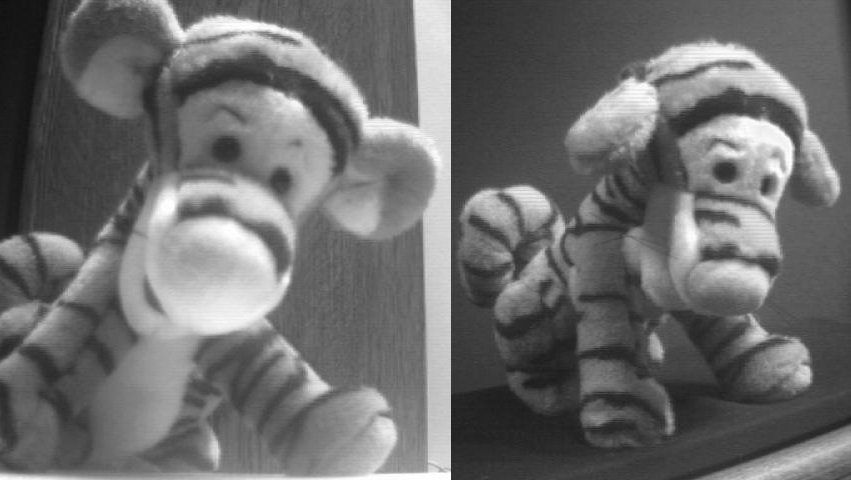
\includegraphics[width=75mm]{figuras/tigger-mit.png}
  \end{center}
  \caption{Brinquedo que responde as emoções das crianças \cite{kirsch1999affective}.}
  \label{fig:tigger-mit}
\end{figure}

O projeto \emph{The Affective Tigger: a reactive expressive toy} de
\citet{kirsch1999affective} é um brinquedo capaz de reconhecer e reagir às
emoções exibidas pelas crianças. Por exemplo, quando a criança encontra-se
feliz, o boneco expressa felicidade (ver Figura~\ref{fig:tigger-mit}). Ao todo
existem 5 estados emocionais: muito feliz, feliz, neutro, triste e muito
triste. Todos, com exceção do neutro, possuem alguma síntese vocal como um
rosnado (tristeza) ou uma risada (muito feliz). Assim, esse brinquedo, por ser
considerado um ser robótico que reage à criança com seus próprios estados
emocionais, fica enquadrado na segunda área.  Portanto, o desenvolvimento
desse brinquedo serviu para aprimorar os seres robóticos.

O projeto AIDA\footnote{Mais detalhes, ver http://senseable.mit.edu/aida} (do
inglês \emph{Affective Intelligent Driving Agent}) pode ser entendido como
enquadrado na área de IHC, pois o interesse é entender o estado afetivo da
pessoa dirigindo. Além disso, interessa-se em ter um relacionamento com o
usuário sugerindo alterações nas rotas baseado na rotina aprendida depois de
um mês de aprendizado.  A pesquisa relatada em \citet{dias-agents} visou
melhorar a simulação de agentes através do uso da emoção guiando o processo
deliberativo e melhorar o entendimento e gerência das emoções.  O presente
trabalho se enquadra na área de síntese de emoção, pois o interesse é em
entender o estado emocional e como ele pode afetar o comportamento de um
personagem.

\section{Modelo Psicológico de Emoção}

Segundo \citet{scherer2000tnoe}, na psicologia há diferentes modelos para
tentar mapear a afetividade: dimensionais, discretos, baseados em significados
e componentes. Os modelos dimensionais procuram estabelecer eixos de classes
de emoções e formas de se mover por esses.  Enquanto os modelos discretos
visam descrever um conjunto básico de emoções ou, ainda, um sistema adaptativo
que evolua a partir de um determinado ponto.  Os modelos baseados em
significados constroem estruturas semânticas e descrevem verbalmente o que
ocorre em determinado sentimento; em outras palavras, preocupa-se com as
situações em que ocasionaram o mesmo. Já os modelos baseados em componentes
entendem que emoções são aprendidas e, sendo assim, estudam o elo entre os
sentimentos e os eventos ou situações que as mesmas acontecem. Esse elo é
montado pela pessoa de diferentes formas.

\citet{Pic98} chama atenção que as emoções sempre foram consideradas um
estigma pela ciência que é fundamentalmente racional com hipóteses testáveis,
argumentos lógicos e experimentos repetitivos.  Entretanto, estudos
neurológicos recentes \cite{ledoux1998emotional,damasio2004erro} mostram a
importância das emoções na tomada de decisão.  \citet{damasio2004erro}
diferencia emoção de sentimento; para ele emoção é um estado físico do corpo e
sentimento é a percepção da mudança desse estado corporal.

\begin{figure*}
  \centering
    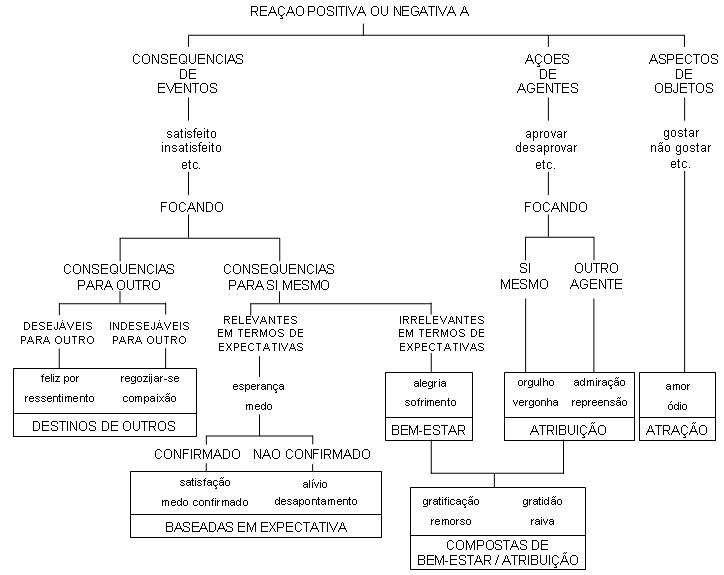
\includegraphics[width=150mm]{figuras/pontarolo_occ.png}
  \caption{Modelo OCC adaptado de \cite{pontarolo2008modelagem}.}
  \label{fig:occ_model_original}
\end{figure*}

O modelo proposto por \citeauthor*{ortony1988cse} \cite{ortony1988cse},
conhecidos na comunidade de Inteligência Artificial, é chamado de OCC por
causa de seus autores.  Esse modelo é classificado como baseado em
significados por descrever as situações de ocorrências de cada uma de suas 22
emoções.  Essas emoções são divididas em formas de se perceber o mundo a sua
volta: Eventos (importantes para alguma meta), Agentes (incluindo a si mesmo)
e Objetos (atração ou repulsa). Assim sendo, essas maneiras de se perceber o
mundo refletem diferentes jeitos de se analisar as situações que podem ser
relativas aos objetivos, valores morais ou gostos da pessoa.

A Figura~\ref{fig:occ_model_original} resume o modelo OCC e mostra as
percepções possíveis de um indivíduo.  Partindo da direita para esquerda, o
ramo mais básico, Aspectos de Objetos, é ativado quando se avalia o gosto de
alguém para algum objeto (inanimado ou não), por exemplo, alguém gostar de
rosas vermelhas.  No seguinte, Ações de agentes, o julgamento das ações
exercidas por outro indivíduo é realizado baseado nos valores morais da pessoa
que está julgando.  Sendo assim, por exemplo, reprovar a atitude de um colega
que ``colou'' na prova. O último da árvore, mais a esquerda, é o de evento que
representa as coisas que aconteceram (e foram consideradas importantes),
acontecem e acontecerão (objetivos almejados). Esses são avaliados segundo as
suas consequências para o alcance ou impedimento dos objetivos de uma pessoa.
Por exemplo, preciso ir bem no concurso para ficar satisfeito porque esse
evento me permitirá alcançar minha meta de ser contratado.

Ainda segundo o modelo OCC, as emoções possuem intensidades. Entretanto, há
distinção entre a valência da emoção e a valência do sentimento. No modelo, um
indivíduo só possui o sentimento quando a intensidade da emoção ultrapassar um
determinado limite.  Essa intensidade é obtida por uma função matemática que
utiliza variáveis de dois tipos: local, que influencia as emoções em um ramo
específico; e global, que influencia todas as emoções do indivíduo.  Um
exemplo de variável local é o desejo, enquanto que um exemplo de variável
global é o senso de realidade.

\section{Ontologias}

\todo{reescrita} Desde Aristóteles, de acordo com \citet{wks2008towards},
começa o estudo das coisas existentes no mundo e a natureza desse existência,
um ramo da filosofia conhecido com ontologia.  Atualmente, na ciência da
computação, ontologias são vistas como um vocabulário de entendimento comum e
compartilhado de um domínio que pode ser utilizada para comunicação entre
pessoas e aplicações distribuídas e heterogêneas.  \citet{ontoly2004Approach}
definem ontologia como uma representação de conhecimento utilizada para
capturar conhecimento e informação sobre determinado assunto, geralmente
estruturado de forma similar a uma rede semântica. Sendo assim, uma ontologia
consiste de um diagrama composto de nodos e arcos que estabelecem uma
fundamentação semântica que permite melhorar a descoberta, interoperabilidade
e reuso do conhecimento.

Logo, o conhecimento pode ser usado de maneiras diferentes e não serve somente
para conter informações em categorias, mas também serve como um tipo de
``banco de dados'' onde instâncias são armazenadas e recuperadas.  O tipo ou
classe da informação possui propriedades que diferem da sua instância. Essa
diferença fica clara quando é feita a comparação da ontologia com uma base de
dados, onde as classes de informações definidas criam as tabelas e as
instâncias povoam os dados nas tabelas.

Na área da computação, ontologias ganharam maior importância com a Web
Semântica permitindo que o conhecimento da página seja facilmente obtido sem
um processamento pesado.  A W3C, orgão internacional que regulamenta padrões
utilizados na Web, regulamentou diversos padrões baseados em \emph{XML} para
ontologias.  A linguagem que será utilizada no presente trabalho será a
OWL\footnote{A sigla vem de ``\emph{Ontology Web Language}''.} e esta fora do
escopo desse artigo aborda-lá em detalhes \footnote{Para mais detalhes, veja
\url{http://www.w3.org/standards/semanticweb/ontology}.}.

\section{Ontologias afetivas}
...

\section{Ontologias de Humanos Virtuais}
...

\section{Trabalhos Relacionados}

O comportamento emotivo do personagem tem um papel importante para se ter a
ilusão de vida conforme afirmou \citet{bates1994role}. Esse trabalho utiliza o
modelo OCC para melhorar a credibilidade dos agentes e cada uma das emoções
pode ser ligada a um comportamento. No exemplo dado anteriormente, um agente
pode ligar o medo a um comportamento agressivo enquanto outro liga essa mesma
emoção de medo a um comportamento de estado alarmado.

\citet{GraCli98} criaram um mecanismo evolucionário utilizando redes neurais
com uma base química para guiar o comportamento do ator. Os atores simulados
podem envelhecer, aprender e, inclusive, se reproduzir (aqui são utilizados
algoritmos genéticos).  Por exemplo, o personagem pode aprender algumas
palavras básicas e demostrar que esta envelhecendo por meio da mudança da cor
de seus cabelos dando uma certa ilusão de vida.

Conforme já dito, as emoções podem melhorar a credibilidade dos seres
virtuais.  \citet{zhang2009emotional} desenvolveram uma aplicação com a
finalidade de demostrar esse conceito. O planejamento das ações a serem
executadas pelo personagem é afetado pelos valores das emoções sendo
experimentadas.

Todos os trabalhos apresentados até aqui, utilizaram as emoções para aumentar
a representação ou expressividade de um ator. Entretanto,
\citet{neto2010construction} tentam estudar o impacto da emoção na decisão dos
agentes.  Assim, para isso ser possível, foi necessário alterar a forma de
planejamento das decisões, além de como recuperar os dados da sua memória.  A
modificação no acesso a memória permite o ``esquecimento'' de determinadas
crenças quando o estado emocional for diferente daquele guardado junto da
memória a ser recuperada. Essa característica torna o planejamento do agente e
as atitudes dos personagens mais realísticas.

\citet{benta2007ontology} e \citet{wks2008towards} descrevem modelos afetivos
através de ontologias. No primeiro trabalho, uma ontologia foi criada
descrevendo emoções primárias e secundárias. O primeiro tipo de emoção exige
menos processamento cognitivo que o segundo. Além disso, o modelo descreve ao
todo 11 emoções sendo 7 dessas consideradas primárias.


\chapter{Arquitetura Emocional Constru\'ida} \label{ch:aec}

\section{Visão Geral}

A presente arquitetura construída foi pensada conforme mostrado na
Figura~\ref{fig:vasc}. Como se pode observar, o sistema é dividido em um
ambiente e em agentes. O ambiente utiliza as ontologias de preferências e de
rotinas para construir a visualização mostrada no capítulo~\ref{ch:cdu}. Dessa
forma, o que o usuário vê é exibido a partir da descrição da ontologia de
rotinas. Mais detalhes ver seção~\ref{ch:aec:ocu}. Já a de preferências,
explicada na seção~\ref{ch:aec:oda}, permite guardar junto dos objetos do
mundo virtual informações quando as mesmas forem estáticas e criar as
preferências dos agentes sobre essas informações.\dev{}
% O dev colocado acima se deve ao fato de a de preferencias ser guardarem
% informacoes, alem das proprias preferencias.

A segunda parte do sistema altera a mente dos atores agindo para acrescentar
anotações em suas percepções e para alterar local que essas crenças são
salvas. A mente dos atores é chamada agente e eles recebem via percepção as suas
preferências e rotinas\dev{}. Essa escolha foi feita para permitir que a
escolha do que fazer seja toda ela escrita em código\dev{} da plataforma
\emph{Jason}. As emoções são concluídas pelo agente através de ontologia
(ver seção~\ref{ch:aec:omce}) e, portanto, a base de crenças padrão da
plataforma foi estendida para consultar, guardar e recuperar os dados
diretamente nessa quando a crença for relevante. Sendo assim, é como se
houvesse dois níveis. O primeiro formado pela ontologia e o segundo pela base
de crença padrão.

\begin{figure}
  \centering
  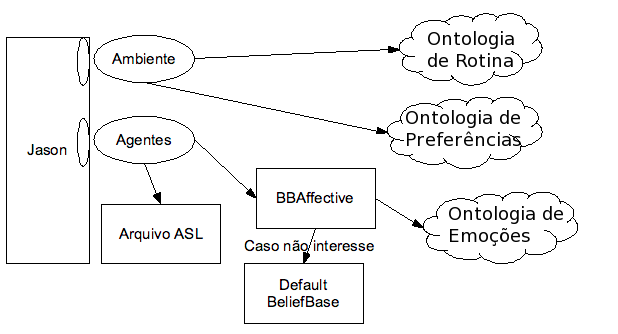
\includegraphics[width=10cm]{figuras/visao-geral.png}
  \caption{Visão abstrata do sistema construído.}
  \label{fig:vasc}
\end{figure}

\section{Ontologia do Modelo Cognitivo Emocional} \label{ch:aec:omce}

A fundamentação do modelo afetivo sendo utilizado aqui é o proposto por
\citet{ortony1988cse} e encontra-se explicado na seção \ref{ch-ca-mce}. A
ontologia proposta tinha como ideia inicial não utilizar regras, porém como
pode ser observado na Tabela~\ref{tab:oa:geral} foi necessário a criação de
regras para suportar o raciocínio no nível de indivíduo corretamente. As
regras que ajudam a conclusão das relações \emph{hasKnow}, \emph{hasFriend} e
\emph{hasEnemy} são diferentes das demais por causa que elas tem como
característica operar no domínio e na imagem da classe \emph{Agent}. Por
exemplo, se John avalia que se relaciona bem com Jose então John
\emph{hasFriend} Jose. Note que o contrario não é necessariamente verdade, o
Jose pode apenas saber que conhece o John então Jose \emph{hasKnow} John.

\begin{table}[h]
	\caption{Ontologia proposta com expressividade: ALCHIN(D).}
	\label{tab:oa:geral}
	\begin{center}
	\begin{tabular}{|c|c|}
	%\begin{tabular}{|p{34mm}|p{50mm}|p{50mm}|}
		\hline
		Descrição & Quantidade \\ \hline
		Classes &  45 		\\ \hline
		Propriedade de Objetos & 16 \\ \hline
		Propriedade de Dados & 14 \\ \hline
		Indivíduos &  0		\\ \hline
		Regras & 7 \\ \hline
	\end{tabular}
	\end{center}
\end{table}

Na Figura~\ref{fig:rlocc} são mostradas as regras desenvolvidas, elas dependem
que os indivíduos da ontologia sejam marcados como diferentes um dos outros.
Assim, recomenda-se fortemente que quando registrar um indivíduo da classe
\emph{Object} ou \emph{Agent} que a informação de igualdade ou diferenciação
seja preenchida\dev{}. Assim, se evita que o raciocinador conclua que não
conhece a resposta e chegue a uma conclusão não esperada.

\begin{figure}[b]
  \centering
  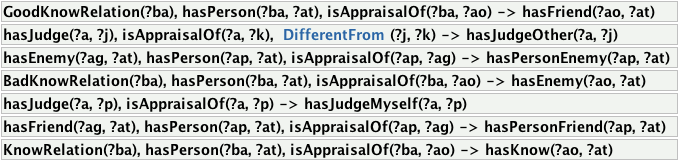
\includegraphics[width=14cm]{figuras/rules-LOCC.png}
  \caption{Regras da ontologia proposta.}
  \label{fig:rlocc}
\end{figure}

A Figura~\ref{fig:kplocc} mostra a árvore de relações que tem como imagem
dados ou instâncias (objetos). Ao se comparar as Figuras~\ref{fig:rlocc}
e \ref{fig:kplocc} se chega a conclusão que as propriedades que as
regras concluem não precisam ser configuradas pelo usuário. Assim, ao invés de
16 propriedades de objetos conforme informado na Tabela~\ref{tab:oa:geral}
apenas 9 precisam ser conhecidas. Dessas, a propriedade menos utilizada é a
\emph{hasSomething} que serve para indicar genericamente o que esta sendo avaliado. Note que
\emph{hasPerson} deve ser usado quando o indivíduo em avaliação for um membro
da classe \emph{Agent}. Já, a relação \emph{hasJudge} serve para indicar que o
membro da classe \emph{Object} esta sendo avaliado pela sua responsabilidade.
Por exemplo, Millie tem uma avaliação julgando seu carro com uma valoração
positiva.

\begin{figure}[b]
  \centering
  \begin{tabular}{cc}
  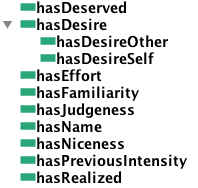
\includegraphics[height=4cm]{figuras/dataProperty-LOCC.png} & 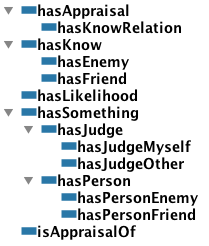
\includegraphics[height=5cm]{figuras/objectProperty-LOCC.png} \\
  (i) Relações de dados & (ii) Relações de Objetos
  \end{tabular}
  \caption{As relações existentes na ontologia proposta.}
  \label{fig:kplocc}
\end{figure}

Todos os dados numéricos da ontologia são inteiros. Isso foi feito com a
finalidade de permitir que o usuário normalize\dev{} o número obtido da
maneira que desejar. Além disso, foi tomada a decisão de não especificar o
domínio da maioria das propriedades por causa que isso forçaria um
enquadramento em classes não desejadas. Por exemplo, se a relação
\emph{hasLikelihood} tiver o domínio \emph{ConsequenceForSelf} e existir um
indivíduo com somente essa relação então o mesmo seria enquadrado no conceito
\emph{ConsequenceForSelf}. Mas, o correto nesse caso seria não ser concluído nada,
ou seja, pertencer à classe \emph{Thing}.

A estrutura da ontologia pode ser visualizada na
Figura~\ref{fig:tlocc}~(pág.~\pageref{fig:tlocc}). Além disso, pode ser
recomendável olhar a
Figura~\ref{fig:occ_model}~(pág.~\pageref{fig:occ_model}) do modelo \occ
durante o resto da discussão dessa seção. Os sub-conceitos de \emph{Emotion}
correspondem aos três ramos do modelo original.
O ramo \emph{ActionsOfAgents} julga a responsabilidade e o quanto o agente que
realizou uma ação ou evento se desviou do esperado, o de
\emph{ConsequencesOfEvents} julga a consequência de um evento e
\emph{AspectsOfObjects} julga a atração para com um objeto.

O primeiro ramo a ser abordado é, o menos cognitivo, \emph{AspectsOfObjects}.
As emoções desse tipo são relacionadas com atratividade e familiaridade.
Entretanto, essas duas relações foram consideradas equivalentes porque o
importante, para o modelo, é quando ambas são positivas ou ambas negativas.
Assim sendo, uma pode assumir os dois papeis sem maiores penalidades e
simplificando a modelagem. A emoção \emph{Hate} é modelada como tendo a
propriedade de familiaridade (\emph{hasFamiliarity}) com valores negativos,
enquanto a emoção \emph{Love} tem valoração dessa mesma propriedade positiva.
Caso o valor seja zero, nada pode ser concluído.

Cabe notar que parece estranho uma emoção \emph{Love} com um objeto, porém
essa emoção foi escolhida por quem montou o modelo para representar seu tipo
por ser a mais forte de sua categoria. Assim, níveis menores implicam em
outros tipos de emoção. Além disso, agentes
podem ser vistos como objetos quando se esta avaliando a sua atração. Logo,
todo agente (\emph{Agent}) é um objeto (\emph{Object}). Por exemplo, John esta
apaixonado pela Millie (\emph{Agent} visto como \emph{Object}) ou John tem
repulsa por televisão.

O segundo conceito, chamado \emph{ActionsOfAgents}, pode ser pensado como
um ramo que julga a responsabilidade por uma determinada ação ou evento.
Assim, esse ramo é capaz de gerar emoções de: Admiração (\emph{Admiration}),
Orgulho (\emph{Pride}), Vergonha (\emph{Shame}) e Reprovação
(\emph{Reproach}). Por exemplo, Jose possui orgulho por cozinhar ou Dilu
reprova Jose porque ele come carne.

Na definição, as emoções de orgulho e vergonha podem acontecer mesmo quando se
esta avaliando ações de outras pessoas. Por exemplo, Dolores tem vergonha de
sua mãe que não cozinha. Essa conclusão é possível por causa de uma relação
que eles propõem de empatia\label{mark:empat}. Entretanto, como em nenhum outro momento, eles
dão mais detalhes sobre essa empatia foi resolvido considerar que vergonha e
orgulho são emoções sentidas somente quando o agente esta avaliando a si mesmo
e, dessa forma, o exemplo anterior não é possível no sistema desenvolvido. \dev{}
% dev -> poderia ter sido usado float e ter feito 1 (para si) e 0 (para outro)

As emoções que julgam responsabilidade são definidas como tendo uma relação de
julgamento (\emph{hasJudge}) e uma relação que mapeia o valor do julgamento
(\emph{hasJudgeness}) que representa o quanto o agente se desviou do
comportamento esperado, isto é, em casos de aprovação é um valor positivo e em
casos de reprovação é um valor negativo. Todavia, isso ainda não permite
diferenciar a emoção de admiração da emoção de orgulho ou a reprovação da de
vergonha. Essa distinção é possível ao se dividir a relação de julgamento com
duas sub-relações: tem auto-julgamento (\emph{hasJudgeMyself}) e tem
julgamento de outro (\emph{hasJudgeOther}).

A utilização de sub-propriedade torna possível escrever a ontologia da maneira
esperada suprimindo o problema. Entretanto, para o usuário pode se tornar
complicado ter que lembrar quando utilizar uma sub-propriedade ou outra.
Assim, foi resolvido deixar o usuário sempre utilizar a relação de julgamento
(\emph{hasJudge}) e via 2 regras inferir se é um auto-julgamento ou o
julgamento de outra pessoa. Para essas regras funcionarem da maneira correta,
o usuário deve declarar que os agentes ou objetos são diferentes uns dos
outros. Caso isso
não ocorra, o sistema considera que não há informação para verificar se um
indivíduo é igual ou diferente e conclui que não conhece a resposta. Além
disso, a relação de julgamento tem como imagem o conceito \emph{Object}. Dessa
forma, os exemplos anteriores são todos válidos.

Cabe salientar que toda avaliação tem pelo menos duas relações. A primeira
relação serve para conhecer quem esta avaliando (\emph{isAppraisalOf}) e a
outra serve para indicar quem ou o que esta sendo avaliado
(\emph{hasSomething}). Essa pode não ser informada explicitamente porque pode
ser concluída quando usada uma de suas sub-relações. O último ramo, chamado de
\emph{ConsequencesOfEvents} é dividido em: \emph{ConsequencesForSelf} e
\emph{ConsequencesForOthers}. Toda essa divisão foca na consequência de um
evento ou ação realizado por algum agente. Por exemplo, Dilu tem pena
de Jose, Jose tem esperança de ser promovido, John tem satisfação por
estar almoçando ou Millie esta alegre por cozinhar.

\begin{wrapfigure}{r}{0.4\textwidth}
  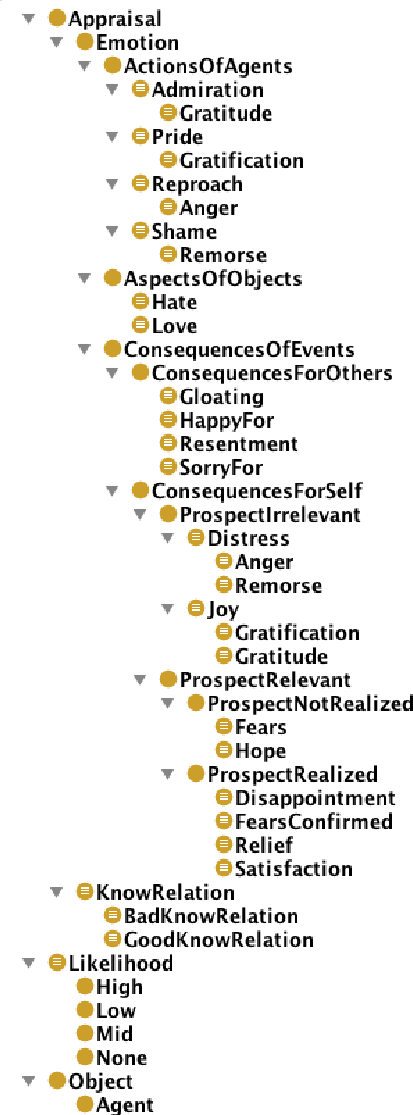
\includegraphics[height=149mm]{figuras/hierarquiaLOCC.png}
  \caption{Taxonomia da ontologia proposta baseado no modelo.}
  \label{fig:tlocc}
\end{wrapfigure}

A \emph{ConsequencesForOthers} expressa 4 emoções: \emph{HappyFor},
\emph{SorryFor}, \emph{Gloating} e \emph{Resentment}. Na definição, essas
emoções dependem: do grau de desejabilidade do avaliador para com o outro; do
grau de desejabilidade que se presume que o outro tenha; do grau de
merecimento do evento; e, do tipo de relacionamento com a pessoa. Na ontologia
proposta, a principal diferença com o modelo \occ é que foi considerado
que o grau de desejabilidade do avaliador para com o outro e o grau de
merecimento do evento são os mesmos. Dessa forma, se pode utilizar apenas três
relações para descrever as 4 emoções.

A relação de merecimento (\emph{hasDeserved}) e de desejabilidade
presumida (\emph{hasDesireOther}) são avaliadas de acordo com sua valoração
positiva ou negativa. A relação \emph{hasPerson} liga o outro indivíduo
sendo avaliado com a avaliação. Para se ter o conhecimento do que esta sendo julgado
ser amigo (\emph{GoodKnowRelation}) ou inimigo (\emph{BadKnowRelation}), esses
conceitos foram criados e precisam ser configurados para cada um dos agentes
em questão. O mesmo pode declarar que só conhece uma pessoa, que conhece e é
um amigo ou que conhece e não gosta dela (inimiga). Entretanto, quem precisa
dessa informação é o conceito de avaliação quando as relações
\emph{hasPersonEnemy} e \emph{hasPersonFriend} precisam ser descobertas.

\emph{ConsequencesForSelf} se divide entre consequências de eventos com
probabilidade relevante (\emph{ProspectRelevant}) e irrelevante
(\emph{ProspectIrrelevant}). Cabe salientar que esses dois conceitos se
relacionam com probabilidade (\emph{hasLikelihood}), entretanto enquanto o
primeiro conceito se relaciona com a parte não nula. A outra se relaciona
somente com essa. Dessa forma, ambos os conceitos são disjuntos. A classe de
probabilidade relevante pode ser dividida ainda entre possibilidade não
realizada (\emph{ProspectNotRealized}) e realizada (\emph{ProspectRealized}).

As emoções \emph{Hope} e \emph{Fear} fazem parte do conceito
\emph{ProspectNotRealized}. Esse conceito usa as relações \emph{hasLikelihood}
e \emph{hasDesireSelf}. Essa última é um número que
representa o desejo de se obter ou repudiar o evento. Além disso, quando o
evento ocorre a emoção atual pode virar uma emoção do conceito
\emph{ProspectRealized}, isto é, \emph{Fear} pode virar ou
\emph{FearsConfirmed} ou \emph{Relief} e \emph{Hope} pode virar ou
\emph{Satisfaction} ou \emph{Disappointment}.

O conceito \emph{ProspectRealized} não se relaciona em nenhum momento com a
relação \emph{hasLikelihood} porque o evento já aconteceu ou não vai mais
acontecer. Assim, ele possui três relações distintas das anteriores, a
primeira é o grau de realização de um evento (\emph{hasRealized}), isto é, a
visão do agente sobre como a consequência do evento aconteceu. A segunda
relação \emph{hasPreviousIntensity} recebe a valoração da emoção de medo ou
esperança do evento que tinha probabilidade e serve para saber se o evento era
um evento bom (esperança) ou ruim (medo). Já, a terceira \emph{hasEffort}
tenta estimar o grau de esforço que foi dispendido para a atração ou repulsa
da consequência do evento.

O conceito \emph{ProspectIrrelevant} é parecido com o conceito
\emph{ProspectRelevant} com a diferença que a relação \emph{hasLikelihood} vai
somente para valores nulos. Fora isso, as emoções desse conceito e do
\emph{ActionsOfAgents} podem ser misturadas formando conceitos compostos.
A composição é quando uma emoção pode ser encaixada em mais de uma emoção
como no caso de se estar alegre (\emph{Joy}), orgulhoso (\emph{Pride}) e
gratificado (\emph{Gratification}). Por fim, o conceito \emph{Setup}
é o utilizado para manter junto da ontologia criada o limite mínimo para uma
emoção virar sentimento\dev{}.

%a transferencia eh feita pelo sistema;
%os dados sao carregados para memoria e eliminados;
%conforme reparado nao ha decaimento da emocao, a mesma eh instantanea;
%2345678901234567890123456789012345678901234567890123456789012345678901234567890

\section{Ontologia de Comportamento Urbano} \label{ch:aec:ocu}

O presente trabalho foca no comportamento de personagens. Dessa forma, uma
ontologia de comportamento urbano tenta descrever a vida normal que um
personagem leva. De outro modo, isso pode ser visto como a rotina regular que
o ator possui em sua cidade virtual.

\begin{figure}
  \centering
    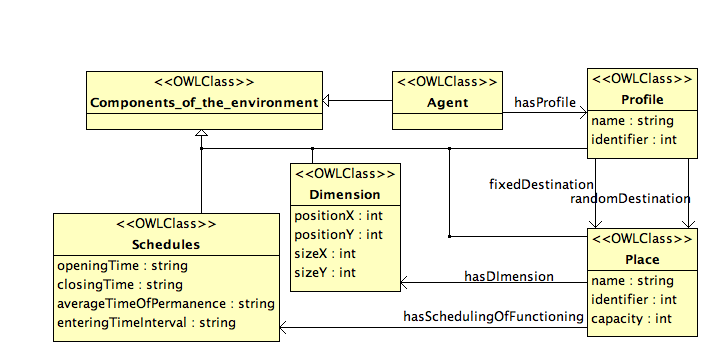
\includegraphics[width=150mm]{figuras/uem-tbox.png}
  \caption[T-Box baseado no modelo de ambiente urbano.]{T-Box baseado no modelo de ambiente urbano \cite{paiva2005ontology}.}
  \label{fig:UEM:TBOX}
\end{figure}

A Figura~\ref{fig:UEM:TBOX} demostra a ontologia, criada por
\citet{paiva2005ontology}, que será utilizada. As relações de generalização
possuem a mesma semântica que na UML, as relações direcionais são relações
binárias entre as instâncias das classes. Na figura, \emph{Agent} se relaciona
com o conceito \emph{Profile} para determinar o tipo de agente. O
\emph{Profile} do agente pode variar entre alguns tipos especificados pelo
usuário que podem possuir destinos fixos (usuais) ou destinos randômicos
(eventuais).

Esses locais são definidos pelo conceito \emph{Place} que contêm
uma descrição de sua capacidade (quantidade máxima de atores), dimensão
(acessível por relação) e horário de funcionamento (acessível por relação). O
conceito de \emph{Dimension} guarda a posição e o tamanho nos eixos X e Y. Já,
o conceito de \emph{Schedules} possui o horário de abertura e fechamento,
intervalo de entrada e tempo médio de permanência.

Além disso, o conceito \emph{Components\_of\_the\_environments} esta sendo
pensando como um sub-conceito de \emph{Setup} na ontologia
desenvolvida por causa que esse representa as configurações gerais.
%
%Essas configurações gerais são carregadas, normalmente, em outras partes do
%sistemas e então eliminadas por causa que elas não influenciam as emoções
%diretamente.
Fora isso, foi introduzido uma nova relação chamada \emph{hasCharacter} que
mapeia o conceito de agente da ontologia anterior para o conceito apresentado aqui.
Dessa forma, um agente na ontologia afetiva pode descobrir seu perfil e descobrir seus locais visitados
regularmente. O conceito de \emph{Place} pode ser pensado, como veremos
adiante, como um ``objeto inteligente''.

Essa ontologia é utilizada no presente trabalho de duas formas. A primeira
forma de utilização é para desenhar um mapa 2D do ambiente que os agentes
atuam. Isso é permitido porque o conceito \emph{Place} relaciona-se com o
\emph{Dimension}. Assim, todos os itens do mapa são retângulos. A outra forma
de utilização é a que trouxe a ontologia para o trabalho e é definir que um
agente tenha sua rotina descrita e disponibilizada pelo ambiente. Para o
ambiente disponibiliza-la via percepção, no ambiente simulado construído cada
dia simulado equivale a aproximadamente 96 ciclos. Isso quer dizer que cada
passo simulado seria em torno de 15 minutos de um dia. Dessa forma, o ambiente
é responsável por conhecer que dia é e informar cada agente de sua rotina para
aquele dia simulado.

\section{Ontologia de Preferências} \label{ch:aec:oda}

\citet{doyle1998annotated} propuseram que o mundo contivesse uma série de
anotações nos objetos. Assim, o agente poderia conhecer apenas a forma de
questionar os objetos sobre suas formas de usar, suas descrições e suas outras
características. Esse conceito veio do conceito \emph{affordance} que se
refere a propriedade de um objeto que dita como o mesmo será utilizado.
Dessa forma, uma cadeira tem a propriedade de ser sentada e uma porta tem as
propriedades de ser aberta ou ser fechada.

Assim, eles utilizaram 5 tipos de anotações: (i) anotações emocionais,
explicam como um agente responde ``emocionalmente''; (ii) anotações de
resposta, explicam como o agente deve reagir ao evento no ambiente que pode ser
uma ação especifica ou uma sugestão de crença; (iii) anotações de resolução de
problemas, descreve o estado do problema e permite anotar dicas que o ator
talvez fale ou realize; (iv) anotações de papel, informam o agente sobre ações
relevantes para determinados trabalhos no mundo; (v) anotações de jogo,
descrevem o estado do jogo permitindo sugerir movimentos.

\citet{kallmann1999modeling} explicaram uma ideia similar, os objetos no mundo
são os responsáveis por proverem para o personagem o como ele deve ser usado.
Por exemplo, durante a animação do personagem estar abrindo uma porta, quem esta
no controle do ator é o ``agente'' que controla a porta. O agente do
personagem delega a responsabilidade da animação para o agente do objeto por
causa que o mesmo é o único que sabe como realizar a animação de abertura ou
fechamento da porta. Esses objetos, denominados objetos inteligentes, precisam
ter um determinado nível de conhecimento sobre o personagem.

De uma maneira similar, o conceito de artefatos que possuem propriedades
observáveis e utilizáveis foi criado por \citet{ricci31cartago}. Por exemplo,
uma porta pode ter como propriedade observável seu estado (estar aberta ou
estar fechada) e ação possível ou propriedade utilizável ser aberta ou ser
fechada. Essas ações podem ficar disponíveis conforme o estado atual do
objeto, mas o controle da disponibilidade e da ação é do próprio objeto por
que é ele que sabe como realizar a ação propriamente dita. O agente unicamente
diz de alguma forma que o objeto tem que realizar tal ação. Nesse trabalho,
não é mencionado que o agente pode ser temporariamente controlado por
objetos.

\begin{figure}
  \centering
    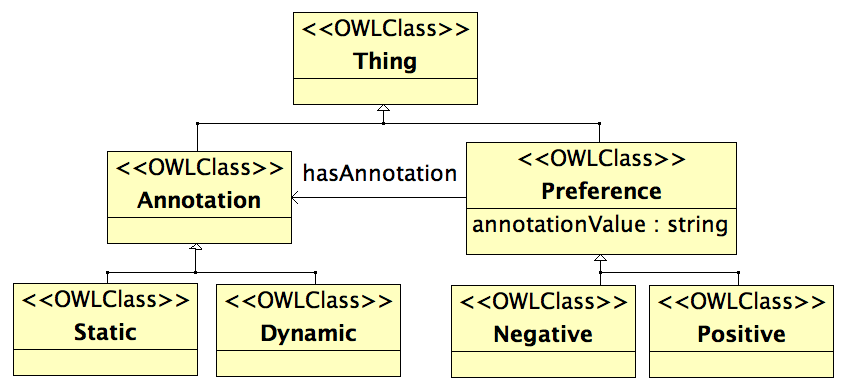
\includegraphics[width=130mm]{figuras/preferences.png}
  \caption{T-Box da ontologia de preferências proposta.}
  \label{fig:preferences}
\end{figure}

A ontologia proposta para as preferências pode ser vista na
Figura~\ref{fig:preferences}. Como pode ser observado, foi criado dois
conceitos principais \emph{Annotation} e \emph{Preference}. O conceito
\emph{Annotation} é utilizado para representar características de determinadas
coisas. Essas características podem ainda ser categorizadas entre as que mudam
e não mudam durante a simulação. O sub-conceito \emph{Dynamic} representa as
características dinâmicas, isto é, as características que podem ser alteradas
durante a ``vida'' do objeto. O sub-conceito \emph{Static} representa as
características que não podem ser alteradas depois da criação do objeto. O
calor e o dono são exemplos de características dinâmicas, enquanto o nome e a
capacidade total são exemplos de características estáticas.

O conceito \emph{Preference} é usado para representar as preferências por
determinadas características ou anotações. A preferência define como uma entidade ou
agente é atraído por determinada característica, por exemplo algumas pessoas
gostam de calor e outras não. Assim, as pessoas que gostam de calor são
atraídas pela valoração positiva da anotação de calor. Já, as pessoas que não
gostam de calor são atraídas pela valoração negativa. Dessa forma, os
sub-conceitos da preferência representam sempre valores que fazem o agente ser
atraído pelo objeto e repelido caso contrário.

Entretanto, esse exemplo não funciona para todos os casos. Por exemplo, um
agente tem conhecimento de seu nível de energia e este é sempre positivo. Para
resolver esse problema foi criada a relação \emph{hasAnnotationValue}
representada na Figura~\ref{fig:preferences} pelo atributo
\emph{annotationValue}. Sendo assim, é possível descrever que um agente com
nível de energia abaixo de um determinado limite é atraído pelo seu centro de
controle.

Essas anotações foram planejadas para serem colocadas pelo ambiente
nos objetos e nos agentes. As anotações em agentes permitem que os outros saibam
o que o agente esta fazendo e como ele parece de forma similar aos objetos. As
preferências também são disponibilizadas em formas de percepção, mas o usuário
que deve criar regras ou planos no \jason para montar as relações usadas pela
afetividade.

\section{Integrando a Plataforma \jason com as ontologias} \label{ch:p:ipjo}

As ontologias explicadas, nas seções anteriores, foram planejadas para serem
usadas como módulos. Sendo assim, as ontologias explicadas anteriormente
podem ser usada sem implicar no uso das demais. Cabe salientar que elas podem ser
usadas tanto pelo agente quanto pelo ambiente conforme poderá ser visto no
capítulo~~\ref{ch:cdu}.

\begin{figure}[b]
  \centering
  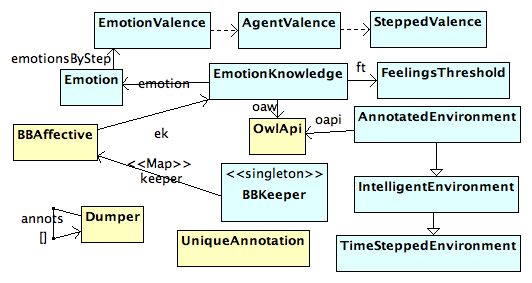
\includegraphics[width=8cm]{figuras/implementacao-15dez2011.png}
  \caption{Diagrama de classes do sistema.}
  \label{fig:dcs}
\end{figure}

Na figura~\ref{fig:dcs} pode ser observado as classes desenvolvidas para
realizar a integração das ontologias com os agentes \jason e o suporte
afetivo. Para essas classes
serem usadas, o agente deve ser configurado para utilizar a classe
\emph{BBAffective} como base de crença. Essas para a implementação da
afetividade funcionar perfeitamente. Essa configuração pode ser feita conforme explicado na
seção~\ref{sec-jason-architecture} (pág.~\pageref{sec-jason-architecture}) e
demostrado na seção~\ref{ch:cdu:tbc} (pág.~\pageref{ch:cdu:tbc}). A classe
\emph{UniqueAnnotation} é a responsável por garantir a não duplicidade de
anotações. %Assim,
%quando se insere por algum motivo duas vezes a mesma anotação apenas valerá a
%última.

A responsabilidade da classe \emph{BBAffective} é manter as crenças dos
agentes e atender as solicitações da plataforma \jason sobre a manipulação
dessas em dois níveis. O primeiro nível é a ontologia e o segundo é a base de
crença padrão que é utilizada quando o elemento não é considerado relevante
para o primeiro nível. A relevância é descoberta consultando os conceitos e
propriedades existentes na ontologia, por exemplo instâncias de conceitos são
crenças no formato ``nomeDoConceito(nomeDaInstancia)'' e relações são
similares à ``nomeDaRelacao(nomeDaInstanciaDominio, Imagem)''. Conhecer o que
é relevante para a ontologia é necessário porque a mesma é lenta e quanto
menos elementos contiver nela melhor será seu desempenho.

A base de crenças delega todo o assunto relacionado com as crenças da
ontologia para a classe \emph{EmotionKnowledge}. Essa é responsável por
conhecer todo o assunto relacionado com as emoções e sentimentos, porém ela
delega o conhecimento da história da potência das emoções para a classe
\emph{Emotion} e o conhecimento dos limites de ativação para a
\emph{FeelingsThreshold}. Da mesma forma, a manipulação e consulta da
ontologia, propriamente dita, é de responsabilidade da classe \emph{OwlApi}.

A classe \emph{Emotion} é responsável por conhecer todas as emoções presentes
e seus valores de potência. Para isso, no inicio da simulação a ontologia é
consultada procurando por todas as classes definidas\footnote{As classes
definidas possuem condições necessárias e suficientes, isto é, qualquer
indivíduo pode ser enquadrado nessa classe desde que obedeça as condições
suficientes.} sobre o conceito ``Emotion''. Isso é utilizado pela classe
\emph{EmotionKnowledge} quando a mesma precisa consultar o nome de uma emoção
por algum motivo. Por exemplo, na hora de calcular a valência da emoção em um
determinado passo é pedido pelo nome de todas as emoções à essa classe. Essa
ainda mantém a história da potência das emoções por agente para cada ciclo
armazenado utilizando um objeto da classe \emph{EmotionValence} que é um
extensão da classe \emph{HashMap} do \emph{Java}.

Para o suporte emotivo funcionar, a classe \emph{FeelingsThreshold} precisa
retornar que todos os limites mínimos de sentimentos estão configurados.
Assim, ela é responsável por fazer essa verificação e por disponibilizar esses
limites para quando for realizado o cálculo da valência. Esse cálculo é
coordenado pela \emph{EmotionKnowledge} que consulta a ontologia, via instância
da classe \emph{OwlApi}, procurando os indivíduos do conceito ``Appraisal''
visando obter as relações de dados desses indivíduos. Dessa forma, a potência
é a soma de todas as propriedades numéricas de um mesmo indivíduo.

As classes de ambiente, isto é, as classes que possuem \emph{Environment} no
nome são responsáveis por diversas coisas relacionadas com o mesmo. Por
exemplo, manter os passos de simulação com um tempo máximo, conhecer a
quantidade de agentes que tem que esperar responderem para ir ao passo de
simulação seguinte, carregar as ações definidas pelo usuário a partir de um
determinado pacote especificado e etc. Cabe salientar, as ações definidas no
ambiente precisam estender a classe \emph{EnvironmentAction} (não desenhada) e
estarem no pacote especificado na chamada a função ``loadAllActions''.

A classe \emph{Dumper} é responsável por conhecer o formato das crenças \jason
e converte-lo para um formato interno. Isso é necessário para proteger o
código feito de mudanças que a plataforma venha a ter. Assim, essa classe é
utilizada por todas as classes internas do sistema e, principalmente, pela
\emph{BBAffective} após constatada a relevância do elemento. Algumas funções
desse tipo são devolver os parâmetros do literal como \emph{string} ou número,
retornar uma instância de seu tipo a partir de um literal, criar o literal a
partir de uma \emph{string} ou a partir de uma outra instância de seu tipo e,
até mesmo, realizar a criação de um \emph{XML} para transferir os dados para
à ontologia.

Já, a classe \emph{BBKeeper} serve para facilitar o acesso a base de crenças.
Essa classe é a única \emph{singleton} do sistema e cada instância da
\emph{BBAffective} é conhecida por esta a partir do nome de seu respectivo
agente. Isso é muito útil para os exemplos porque torna possível acessar a
base de crenças e exibir os valores de potência e valência ou conhecer os
tipos emotivos disponíveis. Cabe salientar que os tipos emotivos disponíveis
do simulador não levam em conta o agente e, por isso, mesmo que seja usado um
agente que não esteja utilizando a base estendida os tipos serão retornados
corretamente.

As seções seguintes, explicam os novos processos de inserção, remoção,
consulta e listagem das crenças. Exemplos desses em código \jason são,
respectivamente, \emph{+crencca}, \emph{-crencca}, \emph{?crencca} e
\emph{?X}. A listagem, também, é utilizada pela tela de visualização de
crenças quando se esta realizando uma depuração no agente.

\subsection{Processo de Listagem e Consulta de Crenças}

\begin{figure}
  \centering
  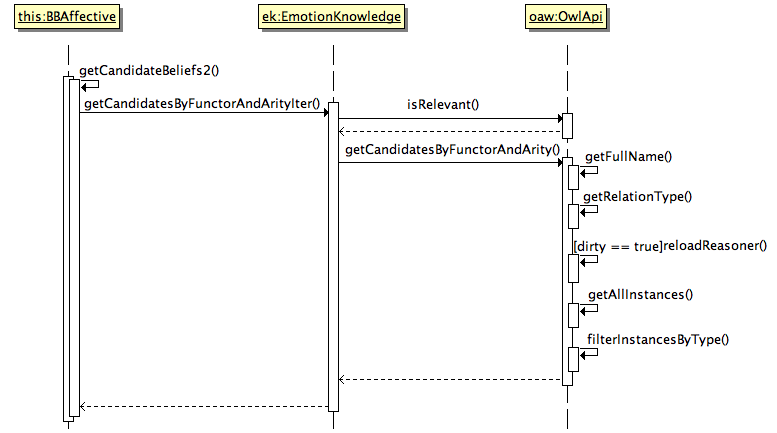
\includegraphics[width=12cm]{figuras/sd-getCB.png}
  \caption{Diagrama de sequência para consultar uma crença.}
  \label{fig:getCandidates}
\end{figure}

O processo de listagem serve para exibir todas as crenças e percepções do
agente. Isso é importante em momentos de depuração ou em momentos que se
deseja consultar uma crença que é uma variável não unificada, isto é, sem
valor definido. Dessa forma, a base de crenças implementa a interface
\emph{java.lang.Iterable} que permite a classe ser usada em construções
\emph{for-each}. A implementação devolve todos os elementos dos dois níveis
sendo que o nível da ontologia é recuperado primeiro.

De maneira similar, o processo de consulta de crenças foi alterado.
%Entretanto, ele pode ser chamado via código \jason ou pelo código \emph{Java}.
Esse processo tem como entrada os métodos com nome \emph{getCandidateBeliefs}
que chamam um método comum denominado \emph{getCandidateBeliefs2} conforme
pode ser visto na Figura~\ref{fig:getCandidates}. O resultado dessa operação é
um objeto \emph{Iterator} com todas as crenças recuperadas da base que possuem
o mesmo nome e mesma aridade que a informada na chamada. Isso é importante
porque esses candidatos podem ter seus parâmetros verificados pela própria
base de crenças ou por outros pontos de acesso do \emph{Jason}.

\subsection{Processo de Recuperação de Crenças}

O processo de recuperação de uma crença é necessário para o entendimento das
inserções e remoções de crenças. Ele serve para recuperar uma única crença
quando ela já existir na base. Esse processo leva em consideração toda a
estrutura do literal, desconsiderando somente as anotações do mesmo em suas
buscas.

A Figura~\ref{fig:recover} mostra esse processo de recuperação. Ele inicia com
a chamada à \emph{getCandidateBeliefs} que foi explicada na seção anterior.
Cada um dos candidatos retornados pela chamada são verificados para ver se
conferem com o informado pelo cliente, se conferir então o candidato é
retornado. Se nenhum candidato for retornado, o resultado da base de crenças
padrão será retornado porque o mesmo pode estar localizado neste nível.
Conforme foi falado anteriormente, tanto a inserção e remoção utilizam esse
procedimento para recuperar o elemento armazenado na base de crença, porém os
motivos serão vistos em suas respectivas seções.

\begin{figure}
  \centering
  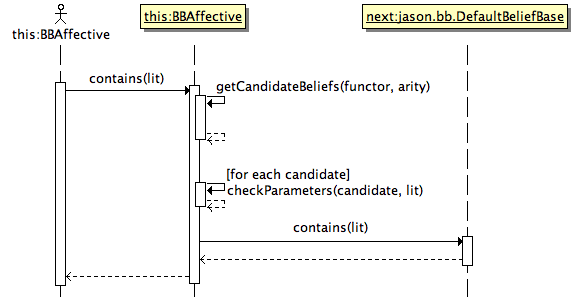
\includegraphics[width=100mm]{figuras/sd-contains.png}
  \caption{Diagrama de sequência para recuperar uma crença.}
  \label{fig:recover}
\end{figure}

\subsection{Processo de Adição de Crenças}

O procedimento de inserção de uma crença pode ser visto na
figura~\ref{fig:addBelief}. Essa figura utiliza as guardas do UML que são
etiquetas com o texto entre colchetes para informar a condição que o código
deve ter para ser executa. Além disso, elas encontram-se localizadas perto de
um quadrado para simbolizar que todas as chamadas feitas dentro deste estão
relacionadas aquelas condições. Dessa forma, quando estiver sendo inserida uma
crença de percepção com o termo diferente de ``step'' nenhum código será
executado pelo diagrama e a mesma será inserida no segundo nível.

A chamada do \jason para a função \emph{add} não se encontra representada na
figura~\ref{fig:addBelief}, porém essa função chama uma outra de mesmo nome e
quando essa retorna falso é chamada a função \emph{add} da instância
\emph{next}. Cabe chamar atenção que quando uma percepção esta sendo inserida
e o termo da crença é ``step'' é realizado o processo de sumarização que
calcula e guarda a potência da emoção na classe \emph{Emotion}. Além disso, se
aproveita o momento para obter e inserir na base de crenças padrão os
sentimentos que acabaram de sofrer atualização em seus valores.

\begin{figure}
  \centering
  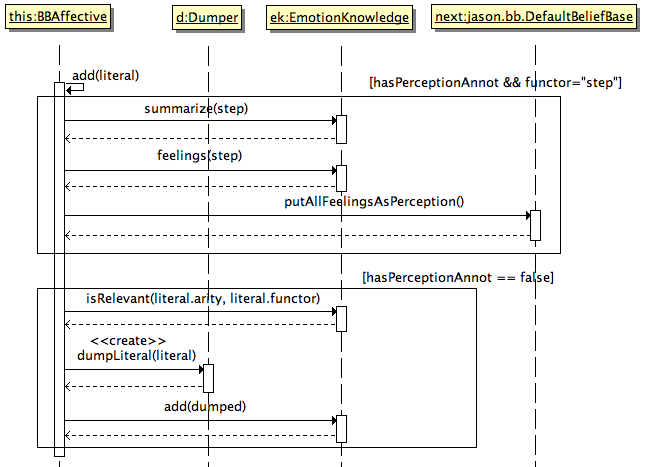
\includegraphics[width=12cm]{figuras/addB.png}
  \caption{Diagrama de sequência para adicionar uma crença.}
  \label{fig:addBelief}
\end{figure}

Agora quando esta sendo feita uma inserção de uma crença que não é uma
percepção, é feita a verificação se ele é relevante. Caso ele seja considerado
irrelevante, a crença sera inserida no segundo nível. Entretanto, se ele for
considerado relevante então será feita a recuperação do elemento atualmente
armazenado e, após isso, é feita a inserção das novas anotações nesse
elemento. Se o elemento não existir na base de crenças então esse último
procedimento é ignorado, porém ele é necessário para haver a correta
atualização das anotações. Por fim, a crença é transformada no tipo interno e
enviado para ser acrescentado na ontologia.

Assim, o processo de inserção serve para inserir os axiomas necessários para
representar essa crença na ontologia quando a mesma for relevante. Para a
criação na ontologia, é necessário ainda diferenciar se é uma instância de
objeto ou propriedade de dados ou de objetos. Essa diferenciação é feita pela
aridade e, em caso de ambiguidade, se pergunta o tipo à ontologia usando o
nome da entidade.

\subsection{Processo de Remoção de Crenças}

O processo de remoção de crenças permite remover uma crença da base de crenças
ou, apenas, atualiza-la retirando alguma anotação que não devia existir. Dessa
forma, o procedimento ao final do mesmo remove os axiomas postos anteriormente
e os insere novamente quando for uma atualização. A Figura~\ref{fig:delBelief}
mostra a rotina da base de crenças.

\begin{figure}
  \centering
  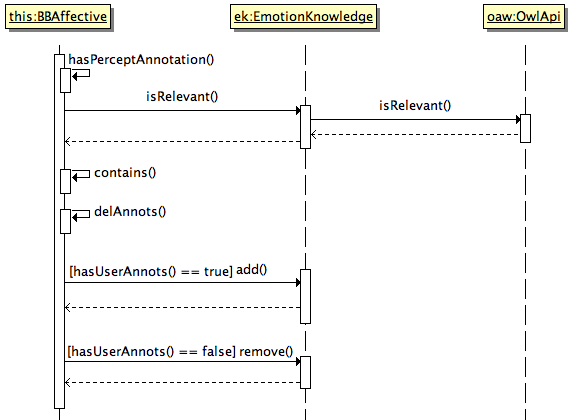
\includegraphics[width=10cm]{figuras/delB.png}
  \caption{Diagrama de sequência para remover uma crença.}
  \label{fig:delBelief}
\end{figure}

A rotina de remoção desenvolvida, inicia verificando se o termo pode ser
considerado relevante. Se ele for uma percepção então ele é irrelevante para
esse procedimento. Caso não seja uma percepção, a relevância é verificada e
se for relevante então é recuperado o elemento armazenado. Se não for
recuperado nenhum elemento ou se ele for irrelevante então é realizada a
chamada a remoção da base de crenças padrão e retornado o resultado.

Nesse momento que se sabe a crença armazenada pelo agente e que a mesma
é relevante. As anotações informadas são removidas da crença obtida e a nova
crença é testada para ver se ainda possui anotações. Se possuir e não for uma
anotação de fonte e não é um indicativo de estar sendo armazenada em
determinada ontologia então é feita a atualização do valor armazenado. No caso
de não possuir anotação ou possuir somente as anotações anteriores mencionadas
é feita a remoção do elemento.

\subsection{Processo Compartilhado de Remoção e Adição de Crenças}

O processo de adição e remoção de crenças compartilham pedaços de códigos. A
classe \emph{EmotionKnowledge} possui dois pontos de entrada, um pelo método
\emph{add} e outro pelo método \emph{remove} tanto um quanto outro fazem uma
chamada para uma função denominada \emph{changeBelief} informando esta se é um
procedimento de inserção ou remoção. A partir dai a sequência de chamadas
mostradas na Figura~\ref{fig:shareBelief} segue de maneira igual. Isso foi
feito porque muito código é igual tanto para um quanto para outra parte.

\begin{figure}
  \centering
  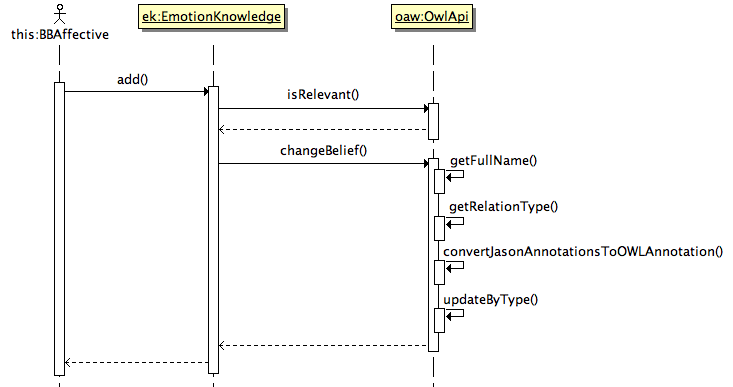
\includegraphics[width=12cm]{figuras/shareBelief.png}
  \caption{Diagrama de sequência para adicionar uma crença.}
  \label{fig:shareBelief}
\end{figure}

A classe \emph{OwlApi} é a única que consulta a ontologia diretamente via
biblioteca. No inicio da aplicação são extraídas as informações de quais
conceitos existem, quais relações e de que tipos elas são. Sendo assim,
consultar o nome completo de uma determinada entidade ou qual é seu tipo não
precisa ir na ontologia. A função \emph{updateByType} é a responsável por
realizar a inserção e remoção das entidades. Uma alteração é feita removendo
a entidade anterior e acrescentando uma nova e marcando a ontologia como suja
para quando uma consulta for feita a mesma ter o raciocinador atualizado.


\chapter{Caso de Uso} \label{ch:cdu}

\todo{comprometimento. Mostrar aqui um arquivo de projeto jason usando opcoes
no agente}

na questao da ontologia de comportamento, acredito q seja possivel
fazer com que um personagem em determinado ciclo vá para um
planeta...

essa questão tras outra pergunta, se um comportamento vai ser
disparado em determinado ciclo para parecer rotina. Quanto tempo,
ou melhor, quantos ciclos representam um dia? E, quanto tempo
é representado por um misero ciclo?

Para responder isso, eu considero o seguinte... eu não vou arredar o
pé de 1000 ciclos. Mas, 1000 estão variando de 4 a 7 minutos reais.
Se considerar que 1000 ciclos possui 10 dias então cada 100 ciclos é um dia.
Dessa forma, usaremos o ciclo equivalente a 870 segundos que correspondem
a 14,5 minutos que equivale a aproximante 99,31 ciclos. Assim, se iniciarmos
o relogio a partir do ciclo 1 no ciclo 100 ou 101 temos uma virada de dia.
Além disso, é importante notar que nem todos os dias viraram no mesmo step.
Por exemplo, alguns vao ter 99 outros 98.... o q torna interessante!

Eu estou pensando em pra ligar com rotinas ter turnos, dividir o dia em
madrugada (24h to 5h30), manha(5h31 to 12h), tarde(12h01 to 18h) e
noite(18h01 to 23h59). Assim, teriamos um turno de 5,5h, outro de 6,5h e os
restantes com 6h.

5 -> Esse tempo pode ser uma percepcao com dia, horario e turno... Simples,
ne?
       E Esse turno `comanda' o que o agente faz no momento porque eh a rotina
       dele, isto eh, pela manha ir em algum lugar amtar gente. Pela tarde
ficar
       matando piratas e a noite/madrugada descansar!

MADRUGADA = M
MANHA = A
TARDE = T
NOITE = N

--
o texto a seguir se refere sempre a ontologia aw.
Nela não temos myself como individuo porque esse
eh um meta individuo para cada ontologia OCC.
Além disso, a alguns atributos novos precisam ser
declarados em ambos. Por exemplo, life que representa
a vida de um personagem. Não existia ate agora,
entretanto a ideia de ter isso visivel como anotacao
pode ser ruim, porém ao inves de life ser visivel aos
outros seria interessante ter visivel damage...
Assim, é interessante pensar no que se quer ver
como exterior e o que se quer ver como myself....
--
Depois disso tem a questão das preferencias ainda,
eu não pensei como nesse nosso ambiente os agentes
vao agir.... eu sei que a maior parte eh mal, gosta de
fazer maldade... alguns são 'companheiros' de outros,
por exemplo podem ver um momento de maldade e
deixar pro colega se divertir...

Outros são excecoes... Vorfield pode ir no planeta
sem matar ninguem, mas a populacao sua não discansa
dessa forma. Ela precisa se afastar... Fora isso o radar dela
 eh melhor com pesos e alcance de 6?


\chapter{Considerações finais}

O presente artigo visa apresentar uma visão do trabalho que está sendo feito
para a construção de um simulador no qual os atores e ambientes interagem.
Entretanto, a ontologia foi omitida porque está ainda sendo aprimorada.  A
idéia apresentada não é nova, porém, o ponto chave é a ontologia permitir aos
agentes raciocinarem sobre suas emoções de forma transparente.  Essa
transparência é útil porque permite ao animador conhecer e, até mesmo,
especificar o personagem com um grau bastante elevado de abstração.
%
Dessa forma, dois agentes com a mesma especificação, ao enfrentarem a mesma
situação, terão o mesmo comportamento quando tiverem vivenciado as mesmas
experiências. Essa experiência inclui as informações adquiridas sobre o
ambiente e sobre os demais atores e não somente os interesses e metas do
mesmo.

O modelo OCC em uso no presente trabalho, foi definido em
\citeyear{ortony1988cse} e possui ao todo 22 emoções especificadas por regras
que demonstram quando a mesma acontece. Entretanto, em nenhum momento da sua
definição foi tratado explicitamente como uma emoção afeta as outras presentes
no personagem.
%
A ferramenta em desenvolvimento tem como interesse a simulação computacional
do comportamento humano e, dessa forma, ela pode ser utilizada de diferentes
maneiras e pode coletar diferentes informações para análises com diversos
propósitos.


%\nocite{*} % Citar todos do arquivo bibtex, mesmo quando nao citado
%\bibliographystyle{abnt-alf} % eh o defauult do abntcite
\bibliography{mestrado}

\end{document}
